% Created 2018-09-26 mer. 02:53
% Intended LaTeX compiler: pdflatex
\documentclass[11pt]{article}
\usepackage[utf8]{inputenc}
\usepackage[T1]{fontenc}
\usepackage{graphicx}
\usepackage{grffile}
\usepackage{longtable}
\usepackage{wrapfig}
\usepackage{rotating}
\usepackage[normalem]{ulem}
\usepackage{amsmath}
\usepackage{textcomp}
\usepackage{amssymb}
\usepackage{capt-of}
\usepackage{hyperref}
\author{teddd}
\date{\today}
\title{}
\hypersetup{
 pdfauthor={teddd},
 pdftitle={},
 pdfkeywords={},
 pdfsubject={},
 pdfcreator={Emacs 26.1 (Org mode 9.1.9)}, 
 pdflang={English}}
\begin{document}

\tableofcontents

\section{Project description}
\label{sec:orgb7ce67a}
\subsection{General Description}
\label{sec:org01a6482}
Goal : Find jobs
\subsubsection{Use}
\label{sec:org54efe86}
\begin{enumerate}
\item target opportunities
\label{sec:orgbe3bb54}
\begin{enumerate}
\item sheets of wanted words
\label{sec:org0e04383}
\item query matching algorithms
\label{sec:org8d898f5}
\end{enumerate}
\item data exploration
\label{sec:org0d9debe}
\item cluster
\label{sec:org30d7d2a}
\begin{enumerate}
\item nlp
\label{sec:org5cba169}
\end{enumerate}
\item find jobs I didn't know about
\label{sec:org2cd533c}
\item get warned if new opportunities
\label{sec:org2e2ace3}
\item use it as a model for finding my perfect match in the world / exploring the economy
\label{sec:orgc649cbb}
\item make it open source and useable by anyone
\label{sec:org6c82733}
\end{enumerate}
\subsubsection{Features}
\label{sec:orge75ba2c}
\begin{enumerate}
\item Update
\label{sec:org621de1c}
\item Clustering
\label{sec:org368aef6}
\item Visualization
\label{sec:org6cd2c05}
\end{enumerate}
\subsection{Plan}
\label{sec:orgb8cf36b}
\subsubsection{Ebay jobs quick scrap}
\label{sec:orgda57c0a}
\begin{enumerate}
\item Think about it while normal digging
\label{sec:org2e91347}
\item Build a simple tool to access the info offline and stay up to date
\label{sec:org26cce1a}
\item List the wanted features and their learning prerequisites
\label{sec:org9c237d5}
\end{enumerate}
\subsubsection{Blogging}
\label{sec:org1e5d11a}
\begin{enumerate}
\item Org babel
\label{sec:org9ab00b4}
\item Website
\label{sec:org06edad6}
\end{enumerate}
\subsubsection{Courses}
\label{sec:org3ac302f}
\begin{enumerate}
\item Databases
\label{sec:org8719737}
\item Visualization
\label{sec:orgd466a07}
\item Machine learning
\label{sec:org2d15798}
\item NLP
\label{sec:orge12bc20}
\item Hash tables / numpy computation
\label{sec:org1a91e83}
\item Proba / stats
\label{sec:orge308461}
\end{enumerate}
\subsubsection{Jobs seeker}
\label{sec:org8b1294c}
\subsection{Implementation}
\label{sec:org6ea7b3a}
\subsubsection{Start a clean project}
\label{sec:org86742d7}
\begin{enumerate}
\item {\bfseries\sffamily TODO} git
\label{sec:org147e883}
\begin{enumerate}
\item a branch per functionality
\label{sec:orgac0617f}
\end{enumerate}
\item {\bfseries\sffamily TODO} projectile
\label{sec:orgd7334e1}
\item file system
\label{sec:orgdd2e52b}
\begin{enumerate}
\item /
\label{sec:org1e04d31}
\begin{enumerate}
\item org
\label{sec:orgfbd2fbd}
\item scraper
\label{sec:org9055bbe}
\item database
\label{sec:org20fe3ac}
\item explorer
\label{sec:orgd82c465}
\end{enumerate}
\end{enumerate}
\item database
\label{sec:org9131b6d}
\begin{enumerate}
\item sql ?
\label{sec:org1cb5daf}
\item csv ?
\label{sec:org1207c4f}
\end{enumerate}
\item org babel file / emacs env
\label{sec:org83e3ae9}
\begin{enumerate}
\item snippets
\label{sec:org5c9eabc}
C-c \& \ldots{}
Tables
C-c C-t is snippet mode for test
\item {\bfseries\sffamily TODO} track time
\label{sec:org9f28b7c}
\item track habits
\label{sec:orgc20b7fe}
\item decide what goes public and what does not at expension
\label{sec:org7818e04}
\end{enumerate}
\end{enumerate}
\section{Explorer}
\label{sec:org2ce1699}
Proper program.
\subsection{Imports}
\label{sec:orgaa834e0}
\subsubsection{ipython}
\label{sec:org99b95eb}
\begin{verbatim}
%matplotlib inline
import matplotlib.pyplot as plt
import numpy as np
\end{verbatim}
\subsubsection{pandas}
\label{sec:org6aae676}
\begin{verbatim}
import pandas as pd    
\end{verbatim}

\subsection{Data load}
\label{sec:orge893e56}
\subsubsection{load everything}
\label{sec:orgbed6642}
\begin{enumerate}
\item file list with path
\label{sec:org68b915c}
\begin{verbatim}
import os
csv_files = []
for dirpath, dirs, files in os.walk("../data/raw"): 
  for filename in files:
    fname = os.path.join(dirpath,filename)
    if fname.endswith('.csv'):
      csv_files.append(fname)
\end{verbatim}

\begin{verbatim}
['bücherei.csv',
'anfänger.csv',
'digital art.csv',
'graphql.log',
'google trends.log',
'jenkins.log',
'cuisine.csv',
'blumen.csv',
'computer vision.csv',
'küchenhilfe.csv',
'scrapping.csv',
'pilzen.csv',
'virtual reality.csv',
'google trends.csv',
'vr.csv',
'computer vision.log',
'mushrooms.csv',
'docker.log',
'advertisment.csv',
'buchhandel.csv',
'flowers.csv',
'digital artist.csv',
'graphql.csv',
'yoga.csv',
'jenkins.csv',
'museum.csv',
'advertisement.csv',
'küche.csv',
'fintech.csv',
'flower.csv',
'movie.csv',
'restaurant.csv',
'crackers.csv',
'docker.csv',
'bio.csv',
'crackers.log',
'garden.csv',
'short movie.csv',
'gardening.csv',
'schneiderei.csv',
'heroku.csv',
'hammam.csv',
'advertisement.log',
'kunst und medien.csv',
'spa.csv']
\end{verbatim}
\item dataframe creation
\label{sec:orgebd2721}
\begin{verbatim}
jobs = pd.DataFrame()

for fl in csv_files:
    print(fl+(30-len(fl)//2)*" *")
    try:
        jobs_set = pd.read_csv(fl)
        jobs_set.dropna(axis=0, how='any', subset=["desc"], inplace=True)
        jobs_set.drop_duplicates(subset="desc", inplace=True)            
        try:                                                             
            jobs.iloc[0,0]                                               
            jobs = jobs.append(jobs_set)                                 
        except IndexError:                                               
            jobs = jobs_set                                              
    except pd.errors.EmptyDataError:
        pass
\end{verbatim}
\item {\bfseries\sffamily TODO} time range selection
\label{sec:org42171fc}
\end{enumerate}
\subsubsection{rename}
\label{sec:org18e32be}
use to quickly reset original df
\begin{verbatim}
df = jobs
\end{verbatim}

\subsubsection{python example\hfill{}\textsc{test}}
\label{sec:org7f2474d}
\begin{verbatim}
x = 12
return x
\end{verbatim}

\begin{verbatim}
return int(x)+1
\end{verbatim}

\subsubsection{org doc elisp example\hfill{}\textsc{test}}
\label{sec:orgd647c97}
\begin{center}
\label{tab:org91470b1}
\begin{tabular}{r}
1\\
2\\
3\\
4\\
\end{tabular}
\end{center}

\begin{verbatim}
(length table)
\end{verbatim}

\subsubsection{python\hfill{}\textsc{python}}
\label{sec:org39cf095}
\begin{verbatim}
"~/data/projects/jobseeker/data/raw/18-09-07/dsp.csv"
\end{verbatim}

\url{None}

\begin{verbatim}
"~/data/projects/jobseeker/data/raw/18-09-07/dsp.csv"
\end{verbatim}

\url{None}

\begin{verbatim}
"~/data/projects/jobseeker/data/raw/18-09-07/python.csv"
\end{verbatim}

\url{None}

\begin{verbatim}
"~/data/projects/jobseeker/data/raw/18-09-07/data scientist.csv"
\end{verbatim}

\url{None}

\begin{verbatim}
"~/data/projects/jobseeker/data/raw/18-09-07/software engineer.csv"
\end{verbatim}

\url{None}
\subsection{Manipulation}
\label{sec:orgee56492}
\subsubsection{Pioneer}
\label{sec:orge2059f0}
\begin{enumerate}
\item get data from path as org variable
\label{sec:orga5dc457}
\begin{verbatim}
import pandas as pd
df = pd.read_csv(data)
\end{verbatim}

\item infos about data
\label{sec:org7a13beb}
\begin{verbatim}
df.count()
\end{verbatim}

\item show short data insight
\label{sec:org6c1be8e}
\begin{enumerate}
\item raw pandas output
\label{sec:org4e31503}
\begin{verbatim}
df.head()
\end{verbatim}
\end{enumerate}

\item browse offers
\label{sec:org25c4026}
\begin{enumerate}
\item add custom function to pretyfy
\label{sec:org798f425}
\begin{verbatim}
from bs4 import BeautifulSoup

def souper(html):
    soup = BeautifulSoup(html, 'html.parser')
    print(soup.get_text())


def soupprint(df, begin, end):
    for i in range(begin, end):
        print(i, df.title.iloc[i])
        print("\n")
        print(df.company.iloc[i])
        print("\n")
        souper(df.desc.iloc[i])
        print("\n"*3)
        print("-"*100)
        print("\n"*3)

\end{verbatim}

\item print it !
\label{sec:org9c475da}
\begin{verbatim}
soupprint(head,0,3)
\end{verbatim}
\end{enumerate}
\end{enumerate}
\subsubsection{cleansing\hfill{}\textsc{clean}}
\label{sec:orge1f14e8}
\begin{enumerate}
\item duplicates
\label{sec:org6af9c4a}
\begin{enumerate}
\item drop\(_{\text{duplicates}}\)
\label{sec:orgefd6bc8}
\begin{verbatim}
df.drop_duplicates(subset="desc", inplace=True)
\end{verbatim}

\item count
\label{sec:org9f70cc1}
\begin{verbatim}
df.title.count()
\end{verbatim}

\begin{verbatim}
11636
\end{verbatim}
\end{enumerate}

\item olders
\label{sec:org454309a}
\begin{enumerate}
\item map lambda\hfill{}\textsc{test}
\label{sec:org075854b}
\begin{verbatim}
df = df[df.days_ago.str.contains("30+").map(lambda x: not x)]
\end{verbatim}

\item \textasciitilde{}\hfill{}\textsc{test}
\label{sec:orgd0347a7}
\begin{verbatim}
df = ~df[df.days_ago.str.contains("30+")]
\end{verbatim}

\item ==False
\label{sec:org8b43d4b}
\begin{verbatim}
df = df[df.days_ago.str.contains("30+")==False]
\end{verbatim}

\item count
\label{sec:org1e597b8}
\begin{verbatim}
len(df)
\end{verbatim}

\begin{verbatim}
5578
\end{verbatim}
\end{enumerate}
\item string numbers to integers
\label{sec:org589ac1c}
\begin{enumerate}
\item sol
\label{sec:orgeb6c721}
\begin{verbatim}
df["days_ago"] = df.days_ago.apply(lambda x: int(x))
\end{verbatim}
\item test
\label{sec:orge122857}
\begin{verbatim}
df.days_ago.iloc[12]
\end{verbatim}

\begin{verbatim}
3
\end{verbatim}
\end{enumerate}
\item drop erratic values
\label{sec:org8fe073c}
\begin{enumerate}
\item run
\label{sec:org5df4b39}
\begin{verbatim}
df = df[df.days_ago.lt(30)]
\end{verbatim}
\item tests
\label{sec:org82cba8b}
\begin{verbatim}
df.days_ago.lt(30)
\end{verbatim}

\begin{verbatim}
3      True
12     True
14     True
15     True
19     True
23     True
27     True
28     True
35     True
38     True
45     True
48     True
55     True
57     True
59     True
62     True
63     True
64     True
65     True
66     True
75     True
79     True
82     True
87     True
91     True
92     True
93     True
94     True
96     True
100    True
...
44     True
46     True
49     True
54     True
55     True
65     True
68     True
69     True
70     True
74     True
77     True
82     True
84     True
87     True
89     True
90     True
93     True
95     True
96     True
97     True
102    True
105    True
109    True
115    True
116    True
119    True
121    True
124    True
126    True
2      True
Name: days_ago, Length: 1625, dtype: bool
\end{verbatim}
\end{enumerate}
\end{enumerate}
\subsubsection{filtering}
\label{sec:orgb34b5bf}
\begin{enumerate}
\item look for keywords
\label{sec:orgb599c0b}
\begin{enumerate}
\item keyword definiton
\label{sec:orgf02269c}
\begin{enumerate}
\item org variable
\label{sec:org844b785}
\begin{verbatim}
"kunst und medien"
\end{verbatim}

kunst und medien
\end{enumerate}

\item look in title
\label{sec:org957a90c}
\begin{enumerate}
\item boolean serie construction\hfill{}\textsc{test}
\label{sec:org63036a4}
\begin{verbatim}
df.title.str.contains(k, case=False)
\end{verbatim}

\begin{verbatim}
3      False
12     False
14     False
15     False
19     False
23     False
27     False
28     False
35     False
38     False
45     False
48     False
55     False
57     False
59     False
62     False
63     False
64     False
65     False
66     False
75     False
79     False
82     False
87     False
91     False
92     False
93     False
94     False
96     False
100    False
...
44     False
46     False
49     False
54     False
55     False
65     False
68     False
69     False
70     False
74     False
77     False
82     False
84     False
87     False
89     False
90     False
93     False
95     False
96     False
97     False
102    False
105    False
109    False
115    False
116    False
119    False
121    False
124    False
126    False
2      False
Name: title, Length: 1623, dtype: bool
\end{verbatim}

\item reduction of our dataset
\label{sec:orgef0c0cd}
\begin{verbatim}
df = df[df.title.str.contains(k, case=False, na=False)]
\end{verbatim}
\end{enumerate}

\item look in description
\label{sec:org503884e}
\begin{verbatim}
df = df[df.desc.str.contains(k, case=False, na=False)]
\end{verbatim}

\item {\bfseries\sffamily TODO} test
\label{sec:orgc2ccdc7}
goto Johnny Kitchin
\begin{verbatim}
k
\end{verbatim}

\begin{verbatim}
"# Out[91]:\n: 'database'"
\end{verbatim}
\end{enumerate}
\item companies
\label{sec:org8df7fbc}
\begin{verbatim}
df = df[df.company.str.contains("berlin", case=False, na=False)]
\end{verbatim}
\end{enumerate}

\subsection{Stats}
\label{sec:orgd193be2}
\subsubsection{overview}
\label{sec:orgbb959bb}
\begin{enumerate}
\item head
\label{sec:org9c402c6}
\begin{verbatim}
df.head()
\end{verbatim}

\begin{verbatim}
Empty DataFrame
Columns: [location, related, title, url, company, days_ago, contract, desc]
Index: []
\end{verbatim}

\item count
\label{sec:org0675d0c}
\begin{verbatim}
len(df)
\end{verbatim}

\begin{verbatim}
0
\end{verbatim}
\end{enumerate}

\subsubsection{days ago}
\label{sec:orgfe8b5e5}
\begin{enumerate}
\item histogram
\label{sec:org9d3db66}
\begin{enumerate}
\item pd plot
\label{sec:org9aa81fb}
\begin{verbatim}
df.days_ago.plot.hist()
\end{verbatim}

\begin{verbatim}
<matplotlib.axes._subplots.AxesSubplot at 0x7f1136869c18>
\end{verbatim}
\begin{center}
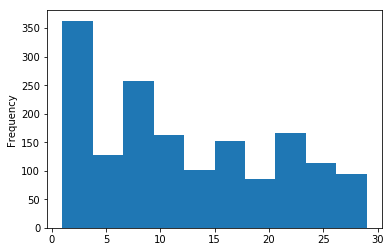
\includegraphics[width=.9\linewidth]{./obipy-resources/TtBMu6.png}
\end{center}
\end{enumerate}
\item value count
\label{sec:org82cfe96}
\begin{verbatim}
df.days_ago.value_counts()
\end{verbatim}

\begin{verbatim}
3     136
1     125
9     115
2     109
8      80
7      74
4      71
10     70
23     68
11     68
14     68
24     57
17     56
16     55
21     55
18     52
15     48
22     47
25     46
28     40
6      39
29     38
13     35
12     28
5      23
27     20
20     19
19     16
26     13
46      1
56      1
Name: days_ago, dtype: int64
\end{verbatim}
\item groupby
\label{sec:orgc07c9cd}
\begin{enumerate}
\item basic output
\label{sec:orgc48f138}
\begin{verbatim}
df.groupby(["days_ago"]).groups
\end{verbatim}

\begin{verbatim}
{1: Int64Index([20, 25, 49, 136], dtype='int64'),
2: Int64Index([2, 4, 10, 30, 71, 77, 116, 125, 139], dtype='int64'),
3: Int64Index([27, 54, 73, 98, 106, 128], dtype='int64'),
4: Int64Index([29, 32, 60, 97, 114, 119, 143], dtype='int64'),
5: Int64Index([50, 135], dtype='int64'),
6: Int64Index([129], dtype='int64'),
7: Int64Index([127], dtype='int64'),
8: Int64Index([104, 112, 113, 121, 138], dtype='int64'),
9: Int64Index([142], dtype='int64'),
10: Int64Index([3, 96], dtype='int64'),
11: Int64Index([86, 132], dtype='int64'),
12: Int64Index([109], dtype='int64'),
13: Int64Index([31], dtype='int64'),
14: Int64Index([22, 24, 95], dtype='int64'),
16: Int64Index([47], dtype='int64'),
17: Int64Index([6, 37, 41], dtype='int64'),
18: Int64Index([80], dtype='int64'),
20: Int64Index([79], dtype='int64'),
21: Int64Index([55], dtype='int64'),
22: Int64Index([1, 144], dtype='int64'),
23: Int64Index([21, 52, 75, 110], dtype='int64'),
24: Int64Index([66, 67], dtype='int64'),
25: Int64Index([14], dtype='int64'),
26: Int64Index([91], dtype='int64'),
27: Int64Index([48], dtype='int64'),
29: Int64Index([145], dtype='int64')}
\end{verbatim}
\item loop print
\label{sec:org969d240}
\begin{verbatim}
grouped = df.groupby("days_ago")

for name,group in grouped:
    print(name)
    print(group)
\end{verbatim}
\item documentation\hfill{}\textsc{doc}
\label{sec:org4676734}
\begin{enumerate}
\item pandas doc
\label{sec:org146c94c}
\begin{verbatim}
help(df.groupby(["days_ago"]))
\end{verbatim}

Help on DataFrameGroupBy in module pandas.core.groupby object:

class DataFrameGroupBy(NDFrameGroupBy)
\begin{center}
\begin{tabular}{l}
Class for grouping and aggregating relational data. See aggregate,\\
transform, and apply functions on this object.\\
\\
It's easiest to use obj.groupby(\ldots{}) to use GroupBy, but you can also do:\\
\\
::\\
\\
grouped = groupby(obj, \ldots{})\\
\\
Parameters\\
----------\\
obj : pandas object\\
axis : int, default 0\\
level : int, default None\\
Level of MultiIndex\\
groupings : list of Grouping objects\\
Most users should ignore this\\
exclusions : array-like, optional\\
List of columns to exclude\\
name : string\\
Most users should ignore this\\
\\
Notes\\
-----\\
After grouping, see aggregate, apply, and transform functions. Here are\\
some other brief notes about usage. When grouping by multiple groups, the\\
result index will be a MultiIndex (hierarchical) by default.\\
\\
Iteration produces (key, group) tuples, i.e. chunking the data by group. So\\
you can write code like:\\
\\
::\\
\\
grouped = obj.groupby(keys, axis=axis)\\
for key, group in grouped:\\
\# do something with the data\\
\\
Function calls on GroupBy, if not specially implemented, "dispatch" to the\\
grouped data. So if you group a DataFrame and wish to invoke the std()\\
method on each group, you can simply do:\\
\\
::\\
\\
df.groupby(mapper).std()\\
\\
rather than\\
\\
::\\
\\
df.groupby(mapper).aggregate(np.std)\\
\\
You can pass arguments to these "wrapped" functions, too.\\
\\
See the online documentation for full exposition on these topics and much\\
more\\
\\
Returns\\
-------\\
\textbf{\textbf{Attributes}}\\
groups : dict\\
\{group name -> group labels\}\\
len(grouped) : int\\
Number of groups\\
\\
Method resolution order:\\
DataFrameGroupBy\\
NDFrameGroupBy\\
GroupBy\\
\_GroupBy\\
pandas.core.base.PandasObject\\
pandas.core.base.StringMixin\\
pandas.core.accessor.DirNamesMixin\\
pandas.core.base.SelectionMixin\\
builtins.object\\
\\
Methods defined here:\\
\\
agg = aggregate(self, arg, *args, **kwargs)\\
\\
aggregate(self, arg, *args, **kwargs)\\
Aggregate using callable, string, dict, or list of string/callables\\
\\
\\
\\
Parameters\\
----------\\
func : callable, string, dictionary, or list of string/callables\\
Function to use for aggregating the data. If a function, must either\\
work when passed a DataFrame or when passed to DataFrame.apply. For\\
a DataFrame, can pass a dict, if the keys are DataFrame column names.\\
\\
Accepted Combinations are:\\
\\
- string function name\\
- function\\
- list of functions\\
- dict of column names -> functions (or list of functions)\\
\\
Notes\\
-----\\
Numpy functions mean/median/prod/sum/std/var are special cased so the\\
default behavior is applying the function along axis=0\\
(e.g., np.mean(arr\(_{\text{2d}}\), axis=0)) as opposed to\\
mimicking the default Numpy behavior (e.g., np.mean(arr\(_{\text{2d}}\))).\\
\\
`agg` is an alias for `aggregate`. Use the alias.\\
\\
Returns\\
-------\\
aggregated : DataFrame\\
\\
Examples\\
--------\\
\\
>>> df = pd.DataFrame(\{'A': [1, 1, 2, 2],\\
\ldots{}                    'B': [1, 2, 3, 4],\\
\ldots{}                    'C': np.random.randn(4)\})\\
\\
>>> df\\
A  B         C\\
0  1  1  0.362838\\
1  1  2  0.227877\\
2  2  3  1.267767\\
3  2  4 -0.562860\\
\\
The aggregation is for each column.\\
\\
>>> df.groupby('A').agg('min')\\
B         C\\
A\\
1  1  0.227877\\
2  3 -0.562860\\
\\
Multiple aggregations\\
\\
>>> df.groupby('A').agg(['min', 'max'])\\
B             C\\
min max       min       max\\
A\\
1   1   2  0.227877  0.362838\\
2   3   4 -0.562860  1.267767\\
\\
Select a column for aggregation\\
\\
>>> df.groupby('A').B.agg(['min', 'max'])\\
min  max\\
A\\
1    1    2\\
2    3    4\\
\\
Different aggregations per column\\
\\
>>> df.groupby('A').agg(\{'B': ['min', 'max'], 'C': 'sum'\})\\
B             C\\
min max       sum\\
A\\
1   1   2  0.590716\\
2   3   4  0.704907\\
\\
See also\\
--------\\
pandas.DataFrame.groupby.apply\\
pandas.DataFrame.groupby.transform\\
pandas.DataFrame.aggregate\\
\\
boxplot = boxplot\(_{\text{frame}}\)\(_{\text{groupby}}\)(grouped, subplots=True, column=None, fontsize=None, rot=0, grid=True, ax=None, figsize=None, layout=None, **kwds)\\
Make box plots from DataFrameGroupBy data.\\
\\
Parameters\\
----------\\
grouped : Grouped DataFrame\\
subplots :\\
* ``False`` - no subplots will be used\\
* ``True`` - create a subplot for each group\\
column : column name or list of names, or vector\\
Can be any valid input to groupby\\
fontsize : int or string\\
rot : label rotation angle\\
grid : Setting this to True will show the grid\\
ax : Matplotlib axis object, default None\\
figsize : A tuple (width, height) in inches\\
layout : tuple (optional)\\
(rows, columns) for the layout of the plot\\
kwds : other plotting keyword arguments to be passed to matplotlib boxplot\\
function\\
\\
Returns\\
-------\\
dict of key/value = group key/DataFrame.boxplot return value\\
or DataFrame.boxplot return value in case subplots=figures=False\\
\\
Examples\\
--------\\
>>> import pandas\\
>>> import numpy as np\\
>>> import itertools\\
>>>\\
>>> tuples = [t for t in itertools.product(range(1000), range(4))]\\
>>> index = pandas.MultiIndex.from\(_{\text{tuples}}\)(tuples, names=['lvl0', 'lvl1'])\\
>>> data = np.random.randn(len(index),4)\\
>>> df = pandas.DataFrame(data, columns=list('ABCD'), index=index)\\
>>>\\
>>> grouped = df.groupby(level='lvl1')\\
>>> boxplot\(_{\text{frame}}\)\(_{\text{groupby}}\)(grouped)\\
>>>\\
>>> grouped = df.unstack(level='lvl1').groupby(level=0, axis=1)\\
>>> boxplot\(_{\text{frame}}\)\(_{\text{groupby}}\)(grouped, subplots=False)\\
\\
count(self)\\
Compute count of group, excluding missing values\\
\\
nunique(self, dropna=True)\\
Return DataFrame with number of distinct observations per group for\\
each column.\\
\\
.. versionadded:: 0.20.0\\
\\
Parameters\\
----------\\
dropna : boolean, default True\\
Don't include NaN in the counts.\\
\\
Returns\\
-------\\
nunique: DataFrame\\
\\
Examples\\
--------\\
>>> df = pd.DataFrame(\{'id': ['spam', 'egg', 'egg', 'spam',\\
\ldots{}                           'ham', 'ham'],\\
\ldots{}                    'value1': [1, 5, 5, 2, 5, 5],\\
\ldots{}                    'value2': list('abbaxy')\})\\
>>> df\\
id  value1 value2\\
0  spam       1      a\\
1   egg       5      b\\
2   egg       5      b\\
3  spam       2      a\\
4   ham       5      x\\
5   ham       5      y\\
\\
>>> df.groupby('id').nunique()\\
id  value1  value2\\
id\\
egg    1       1       1\\
ham    1       1       2\\
spam   1       2       1\\
\\
\# check for rows with the same id but conflicting values\\
>>> df.groupby('id').filter(lambda g: (g.nunique() > 1).any())\\
id  value1 value2\\
0  spam       1      a\\
3  spam       2      a\\
4   ham       5      x\\
5   ham       5      y\\
\\
----------------------------------------------------------------------\\
Data descriptors defined here:\\
\\
all\\
\\
Return whether all elements are True over requested axis\\
\\
Parameters\\
----------\\
axis : \{index (0), columns (1)\}\\
skipna : boolean, default True\\
Exclude NA/null values. If an entire row/column is NA, the result\\
will be NA\\
level : int or level name, default None\\
If the axis is a MultiIndex (hierarchical), count along a\\
particular level, collapsing into a Series\\
bool\(_{\text{only}}\) : boolean, default None\\
Include only boolean columns. If None, will attempt to use everything,\\
then use only boolean data. Not implemented for Series.\\
\\
Returns\\
-------\\
all : Series or DataFrame (if level specified)\\
\\
any\\
\\
Return whether any element is True over requested axis\\
\\
Parameters\\
----------\\
axis : \{index (0), columns (1)\}\\
skipna : boolean, default True\\
Exclude NA/null values. If an entire row/column is NA, the result\\
will be NA\\
level : int or level name, default None\\
If the axis is a MultiIndex (hierarchical), count along a\\
particular level, collapsing into a Series\\
bool\(_{\text{only}}\) : boolean, default None\\
Include only boolean columns. If None, will attempt to use everything,\\
then use only boolean data. Not implemented for Series.\\
\\
Returns\\
-------\\
any : Series or DataFrame (if level specified)\\
\\
corr\\
Compute pairwise correlation of columns, excluding NA/null values\\
\\
Parameters\\
----------\\
method : \{'pearson', 'kendall', 'spearman'\}\\
* pearson : standard correlation coefficient\\
* kendall : Kendall Tau correlation coefficient\\
* spearman : Spearman rank correlation\\
min\(_{\text{periods}}\) : int, optional\\
Minimum number of observations required per pair of columns\\
to have a valid result. Currently only available for pearson\\
and spearman correlation\\
\\
Returns\\
-------\\
y : DataFrame\\
\\
corrwith\\
Compute pairwise correlation between rows or columns of two DataFrame\\
objects.\\
\\
Parameters\\
----------\\
other : DataFrame\\
axis : \{0 or 'index', 1 or 'columns'\}, default 0\\
0 or 'index' to compute column-wise, 1 or 'columns' for row-wise\\
drop : boolean, default False\\
Drop missing indices from result, default returns union of all\\
\\
Returns\\
-------\\
correls : Series\\
\\
cov\\
Compute pairwise covariance of columns, excluding NA/null values\\
\\
Parameters\\
----------\\
min\(_{\text{periods}}\) : int, optional\\
Minimum number of observations required per pair of columns\\
to have a valid result.\\
\\
Returns\\
-------\\
y : DataFrame\\
\\
Notes\\
-----\\
`y` contains the covariance matrix of the DataFrame's time series.\\
The covariance is normalized by N-1 (unbiased estimator).\\
\\
diff\\
1st discrete difference of object\\
\\
Parameters\\
----------\\
periods : int, default 1\\
Periods to shift for forming difference\\
axis : \{0 or 'index', 1 or 'columns'\}, default 0\\
Take difference over rows (0) or columns (1).\\
\\
.. versionadded: 0.16.1\\
\\
Returns\\
-------\\
diffed : DataFrame\\
\\
dtypes\\
Return the dtypes in this object.\\
\\
fillna\\
Fill NA/NaN values using the specified method\\
\\
Parameters\\
----------\\
value : scalar, dict, Series, or DataFrame\\
Value to use to fill holes (e.g. 0), alternately a\\
dict/Series/DataFrame of values specifying which value to use for\\
each index (for a Series) or column (for a DataFrame). (values not\\
in the dict/Series/DataFrame will not be filled). This value cannot\\
be a list.\\
method : \{'backfill', 'bfill', 'pad', 'ffill', None\}, default None\\
Method to use for filling holes in reindexed Series\\
pad / ffill: propagate last valid observation forward to next valid\\
backfill / bfill: use NEXT valid observation to fill gap\\
axis : \{0 or 'index', 1 or 'columns'\}\\
inplace : boolean, default False\\
If True, fill in place. Note: this will modify any\\
other views on this object, (e.g. a no-copy slice for a column in a\\
DataFrame).\\
limit : int, default None\\
If method is specified, this is the maximum number of consecutive\\
NaN values to forward/backward fill. In other words, if there is\\
a gap with more than this number of consecutive NaNs, it will only\\
be partially filled. If method is not specified, this is the\\
maximum number of entries along the entire axis where NaNs will be\\
filled. Must be greater than 0 if not None.\\
downcast : dict, default is None\\
a dict of item->dtype of what to downcast if possible,\\
or the string 'infer' which will try to downcast to an appropriate\\
equal type (e.g. float64 to int64 if possible)\\
\\
See Also\\
--------\\
reindex, asfreq\\
\\
Returns\\
-------\\
filled : DataFrame\\
\\
Examples\\
--------\\
>>> df = pd.DataFrame([[np.nan, 2, np.nan, 0],\\
\ldots{}                    [3, 4, np.nan, 1],\\
\ldots{}                    [np.nan, np.nan, np.nan, 5],\\
\ldots{}                    [np.nan, 3, np.nan, 4]],\\
\ldots{}                    columns=list('ABCD'))\\
>>> df\\
A    B   C  D\\
0  NaN  2.0 NaN  0\\
1  3.0  4.0 NaN  1\\
2  NaN  NaN NaN  5\\
3  NaN  3.0 NaN  4\\
\\
Replace all NaN elements with 0s.\\
\\
>>> df.fillna(0)\\
A   B   C   D\\
0   0.0 2.0 0.0 0\\
1   3.0 4.0 0.0 1\\
2   0.0 0.0 0.0 5\\
3   0.0 3.0 0.0 4\\
\\
We can also propagate non-null values forward or backward.\\
\\
>>> df.fillna(method='ffill')\\
A   B   C   D\\
0   NaN 2.0 NaN 0\\
1   3.0 4.0 NaN 1\\
2   3.0 4.0 NaN 5\\
3   3.0 3.0 NaN 4\\
\\
Replace all NaN elements in column 'A', 'B', 'C', and 'D', with 0, 1,\\
2, and 3 respectively.\\
\\
>>> values = \{'A': 0, 'B': 1, 'C': 2, 'D': 3\}\\
>>> df.fillna(value=values)\\
A   B   C   D\\
0   0.0 2.0 2.0 0\\
1   3.0 4.0 2.0 1\\
2   0.0 1.0 2.0 5\\
3   0.0 3.0 2.0 4\\
\\
Only replace the first NaN element.\\
\\
>>> df.fillna(value=values, limit=1)\\
A   B   C   D\\
0   0.0 2.0 2.0 0\\
1   3.0 4.0 NaN 1\\
2   NaN 1.0 NaN 5\\
3   NaN 3.0 NaN 4\\
\\
hist\\
Draw histogram of the DataFrame's series using matplotlib / pylab.\\
\\
Parameters\\
----------\\
data : DataFrame\\
column : string or sequence\\
If passed, will be used to limit data to a subset of columns\\
by : object, optional\\
If passed, then used to form histograms for separate groups\\
grid : boolean, default True\\
Whether to show axis grid lines\\
xlabelsize : int, default None\\
If specified changes the x-axis label size\\
xrot : float, default None\\
rotation of x axis labels\\
ylabelsize : int, default None\\
If specified changes the y-axis label size\\
yrot : float, default None\\
rotation of y axis labels\\
ax : matplotlib axes object, default None\\
sharex : boolean, default True if ax is None else False\\
In case subplots=True, share x axis and set some x axis labels to\\
invisible; defaults to True if ax is None otherwise False if an ax\\
is passed in; Be aware, that passing in both an ax and sharex=True\\
will alter all x axis labels for all subplots in a figure!\\
sharey : boolean, default False\\
In case subplots=True, share y axis and set some y axis labels to\\
invisible\\
figsize : tuple\\
The size of the figure to create in inches by default\\
layout : tuple, optional\\
Tuple of (rows, columns) for the layout of the histograms\\
bins : integer, default 10\\
Number of histogram bins to be used\\
kwds : other plotting keyword arguments\\
To be passed to hist function\\
\\
idxmax\\
Return index of first occurrence of maximum over requested axis.\\
NA/null values are excluded.\\
\\
Parameters\\
----------\\
axis : \{0 or 'index', 1 or 'columns'\}, default 0\\
0 or 'index' for row-wise, 1 or 'columns' for column-wise\\
skipna : boolean, default True\\
Exclude NA/null values. If an entire row/column is NA, the result\\
will be NA.\\
\\
Raises\\
------\\
ValueError\\
* If the row/column is empty\\
\\
Returns\\
-------\\
idxmax : Series\\
\\
Notes\\
-----\\
This method is the DataFrame version of ``ndarray.argmax``.\\
\\
See Also\\
--------\\
Series.idxmax\\
\\
idxmin\\
Return index of first occurrence of minimum over requested axis.\\
NA/null values are excluded.\\
\\
Parameters\\
----------\\
axis : \{0 or 'index', 1 or 'columns'\}, default 0\\
0 or 'index' for row-wise, 1 or 'columns' for column-wise\\
skipna : boolean, default True\\
Exclude NA/null values. If an entire row/column is NA, the result\\
will be NA.\\
\\
Raises\\
------\\
ValueError\\
* If the row/column is empty\\
\\
Returns\\
-------\\
idxmin : Series\\
\\
Notes\\
-----\\
This method is the DataFrame version of ``ndarray.argmin``.\\
\\
See Also\\
--------\\
Series.idxmin\\
\\
mad\\
\\
Return the mean absolute deviation of the values for the requested axis\\
\\
Parameters\\
----------\\
axis : \{index (0), columns (1)\}\\
skipna : boolean, default True\\
Exclude NA/null values when computing the result.\\
level : int or level name, default None\\
If the axis is a MultiIndex (hierarchical), count along a\\
particular level, collapsing into a Series\\
numeric\(_{\text{only}}\) : boolean, default None\\
Include only float, int, boolean columns. If None, will attempt to use\\
everything, then use only numeric data. Not implemented for Series.\\
\\
Returns\\
-------\\
mad : Series or DataFrame (if level specified)\\
\\
pct\(_{\text{change}}\)\\
Percent change over given number of periods.\\
\\
Parameters\\
----------\\
periods : int, default 1\\
Periods to shift for forming percent change\\
fill\(_{\text{method}}\) : str, default 'pad'\\
How to handle NAs before computing percent changes\\
limit : int, default None\\
The number of consecutive NAs to fill before stopping\\
freq : DateOffset, timedelta, or offset alias string, optional\\
Increment to use from time series API (e.g. 'M' or BDay())\\
\\
Returns\\
-------\\
chg : NDFrame\\
\\
Notes\\
-----\\
\\
By default, the percentage change is calculated along the stat\\
axis: 0, or ``Index``, for ``DataFrame`` and 1, or ``minor`` for\\
``Panel``. You can change this with the ``axis`` keyword argument.\\
\\
quantile\\
Return values at the given quantile over requested axis, a la\\
numpy.percentile.\\
\\
Parameters\\
----------\\
q : float or array-like, default 0.5 (50\% quantile)\\
0 <= q <= 1, the quantile(s) to compute\\
axis : \{0, 1, 'index', 'columns'\} (default 0)\\
0 or 'index' for row-wise, 1 or 'columns' for column-wise\\
interpolation : \{'linear', 'lower', 'higher', 'midpoint', 'nearest'\}\\
.. versionadded:: 0.18.0\\
\\
This optional parameter specifies the interpolation method to use,\\
when the desired quantile lies between two data points `i` and `j`:\\
\\
* linear: `i + (j - i) * fraction`, where `fraction` is the\\
fractional part of the index surrounded by `i` and `j`.\\
* lower: `i`.\\
* higher: `j`.\\
* nearest: `i` or `j` whichever is nearest.\\
* midpoint: (`i` + `j`) / 2.\\
\\
Returns\\
-------\\
quantiles : Series or DataFrame\\
\\
- If ``q`` is an array, a DataFrame will be returned where the\\
index is ``q``, the columns are the columns of self, and the\\
values are the quantiles.\\
- If ``q`` is a float, a Series will be returned where the\\
index is the columns of self and the values are the quantiles.\\
\\
Examples\\
--------\\
\\
>>> df = DataFrame(np.array([[1, 1], [2, 10], [3, 100], [4, 100]]),\\
columns=['a', 'b'])\\
>>> df.quantile(.1)\\
a    1.3\\
b    3.7\\
dtype: float64\\
>>> df.quantile([.1, .5])\\
a     b\\
0.1  1.3   3.7\\
0.5  2.5  55.0\\
\\
rank\\
Compute numerical data ranks (1 through n) along axis. Equal values are\\
assigned a rank that is the average of the ranks of those values\\
\\
Parameters\\
----------\\
axis : \{0 or 'index', 1 or 'columns'\}, default 0\\
index to direct ranking\\
method : \{'average', 'min', 'max', 'first', 'dense'\}\\
* average: average rank of group\\
* min: lowest rank in group\\
* max: highest rank in group\\
* first: ranks assigned in order they appear in the array\\
* dense: like 'min', but rank always increases by 1 between groups\\
numeric\(_{\text{only}}\) : boolean, default None\\
Include only float, int, boolean data. Valid only for DataFrame or\\
Panel objects\\
na\(_{\text{option}}\) : \{'keep', 'top', 'bottom'\}\\
* keep: leave NA values where they are\\
* top: smallest rank if ascending\\
* bottom: smallest rank if descending\\
ascending : boolean, default True\\
False for ranks by high (1) to low (N)\\
pct : boolean, default False\\
Computes percentage rank of data\\
\\
Returns\\
-------\\
ranks : same type as caller\\
\\
skew\\
\\
Return unbiased skew over requested axis\\
Normalized by N-1\\
\\
Parameters\\
----------\\
axis : \{index (0), columns (1)\}\\
skipna : boolean, default True\\
Exclude NA/null values when computing the result.\\
level : int or level name, default None\\
If the axis is a MultiIndex (hierarchical), count along a\\
particular level, collapsing into a Series\\
numeric\(_{\text{only}}\) : boolean, default None\\
Include only float, int, boolean columns. If None, will attempt to use\\
everything, then use only numeric data. Not implemented for Series.\\
\\
Returns\\
-------\\
skew : Series or DataFrame (if level specified)\\
\\
take\\
Return the elements in the given \textbf{positional} indices along an axis.\\
\\
This means that we are not indexing according to actual values in\\
the index attribute of the object. We are indexing according to the\\
actual position of the element in the object.\\
\\
Parameters\\
----------\\
indices : array-like\\
An array of ints indicating which positions to take.\\
axis : int, default 0\\
The axis on which to select elements. "0" means that we are\\
selecting rows, "1" means that we are selecting columns, etc.\\
convert : bool, default True\\
.. deprecated:: 0.21.0\\
In the future, negative indices will always be converted.\\
\\
Whether to convert negative indices into positive ones.\\
For example, ``-1`` would map to the ``len(axis) - 1``.\\
The conversions are similar to the behavior of indexing a\\
regular Python list.\\
is\(_{\text{copy}}\) : bool, default True\\
Whether to return a copy of the original object or not.\\
\\
Examples\\
--------\\
>>> df = pd.DataFrame([('falcon', 'bird',    389.0),\\
('parrot', 'bird',     24.0),\\
('lion',   'mammal',   80.5),\\
('monkey', 'mammal', np.nan)],\\
columns=('name', 'class', 'max\(_{\text{speed}}\)'),\\
index=[0, 2, 3, 1])\\
>>> df\\
name   class  max\(_{\text{speed}}\)\\
0  falcon    bird      389.0\\
2  parrot    bird       24.0\\
3    lion  mammal       80.5\\
1  monkey  mammal        NaN\\
\\
Take elements at positions 0 and 3 along the axis 0 (default).\\
\\
Note how the actual indices selected (0 and 1) do not correspond to\\
our selected indices 0 and 3. That's because we are selecting the 0th\\
and 3rd rows, not rows whose indices equal 0 and 3.\\
\\
>>> df.take([0, 3])\\
0  falcon    bird      389.0\\
1  monkey  mammal        NaN\\
\\
Take elements at indices 1 and 2 along the axis 1 (column selection).\\
\\
>>> df.take([1, 2], axis=1)\\
class  max\(_{\text{speed}}\)\\
0    bird      389.0\\
2    bird       24.0\\
3  mammal       80.5\\
1  mammal        NaN\\
\\
We may take elements using negative integers for positive indices,\\
starting from the end of the object, just like with Python lists.\\
\\
>>> df.take([-1, -2])\\
name   class  max\(_{\text{speed}}\)\\
1  monkey  mammal        NaN\\
3    lion  mammal       80.5\\
\\
Returns\\
-------\\
taken : type of caller\\
An array-like containing the elements taken from the object.\\
\\
See Also\\
--------\\
numpy.ndarray.take\\
numpy.take\\
\\
tshift\\
Shift the time index, using the index's frequency if available.\\
\\
Parameters\\
----------\\
periods : int\\
Number of periods to move, can be positive or negative\\
freq : DateOffset, timedelta, or time rule string, default None\\
Increment to use from the tseries module or time rule (e.g. 'EOM')\\
axis : int or basestring\\
Corresponds to the axis that contains the Index\\
\\
Notes\\
-----\\
If freq is not specified then tries to use the freq or inferred\(_{\text{freq}}\)\\
attributes of the index. If neither of those attributes exist, a\\
ValueError is thrown\\
\\
Returns\\
-------\\
shifted : NDFrame\\
\\
----------------------------------------------------------------------\\
Methods inherited from NDFrameGroupBy:\\
\\
filter(self, func, dropna=True, *args, **kwargs)\\
Return a copy of a DataFrame excluding elements from groups that\\
do not satisfy the boolean criterion specified by func.\\
\\
Parameters\\
----------\\
f : function\\
Function to apply to each subframe. Should return True or False.\\
dropna : Drop groups that do not pass the filter. True by default;\\
if False, groups that evaluate False are filled with NaNs.\\
\\
Notes\\
-----\\
Each subframe is endowed the attribute 'name' in case you need to know\\
which group you are working on.\\
\\
Examples\\
--------\\
>>> import pandas as pd\\
>>> df = pd.DataFrame(\{'A' : ['foo', 'bar', 'foo', 'bar',\\
\ldots{}                           'foo', 'bar'],\\
\ldots{}                    'B' : [1, 2, 3, 4, 5, 6],\\
\ldots{}                    'C' : [2.0, 5., 8., 1., 2., 9.]\})\\
>>> grouped = df.groupby('A')\\
>>> grouped.filter(lambda x: x['B'].mean() > 3.)\\
A  B    C\\
1  bar  2  5.0\\
3  bar  4  1.0\\
5  bar  6  9.0\\
\\
Returns\\
-------\\
filtered : DataFrame\\
\\
transform(self, func, *args, **kwargs)\\
Call function producing a like-indexed DataFrame on each group and\\
return a DataFrame having the same indexes as the original object\\
filled with the transformed values\\
\\
Parameters\\
----------\\
f : function\\
Function to apply to each group\\
\\
Notes\\
-----\\
Each group is endowed the attribute 'name' in case you need to know\\
which group you are working on.\\
\\
The current implementation imposes three requirements on f:\\
\\
* f must return a value that either has the same shape as the input\\
subframe or can be broadcast to the shape of the input subframe.\\
For example, f returns a scalar it will be broadcast to have the\\
same shape as the input subframe.\\
* if this is a DataFrame, f must support application column-by-column\\
in the subframe. If f also supports application to the entire subframe,\\
then a fast path is used starting from the second chunk.\\
* f must not mutate groups. Mutation is not supported and may\\
produce unexpected results.\\
\\
Returns\\
-------\\
DataFrame\\
\\
See also\\
--------\\
aggregate, transform\\
\\
Examples\\
--------\\
\\
\# Same shape\\
>>> df = pd.DataFrame(\{'A' : ['foo', 'bar', 'foo', 'bar',\\
\ldots{}                           'foo', 'bar'],\\
\ldots{}                    'B' : ['one', 'one', 'two', 'three',\\
\ldots{}                          'two', 'two'],\\
\ldots{}                    'C' : [1, 5, 5, 2, 5, 5],\\
\ldots{}                    'D' : [2.0, 5., 8., 1., 2., 9.]\})\\
>>> grouped = df.groupby('A')\\
>>> grouped.transform(lambda x: (x - x.mean()) / x.std())\\
C         D\\
0 -1.154701 -0.577350\\
1  0.577350  0.000000\\
2  0.577350  1.154701\\
3 -1.154701 -1.000000\\
4  0.577350 -0.577350\\
5  0.577350  1.000000\\
\\
\# Broadcastable\\
>>> grouped.transform(lambda x: x.max() - x.min())\\
C    D\\
0  4  6.0\\
1  3  8.0\\
2  4  6.0\\
3  3  8.0\\
4  4  6.0\\
5  3  8.0\\
\\
----------------------------------------------------------------------\\
Methods inherited from GroupBy:\\
\\
backfill(self, limit=None)\\
Backward fill the values\\
\\
Parameters\\
----------\\
limit : integer, optional\\
limit of how many values to fill\\
\\
See Also\\
--------\\
Series.fillna\\
DataFrame.fillna\\
\\
\\
See also\\
--------\\
pandas.Series.groupby\\
pandas.DataFrame.groupby\\
pandas.Panel.groupby\\
\\
bfill = backfill(self, limit=None)\\
Backward fill the values\\
\\
Parameters\\
----------\\
limit : integer, optional\\
limit of how many values to fill\\
\\
See Also\\
--------\\
Series.fillna\\
DataFrame.fillna\\
\\
\\
See also\\
--------\\
pandas.Series.groupby\\
pandas.DataFrame.groupby\\
pandas.Panel.groupby\\
\\
cumcount(self, ascending=True)\\
Number each item in each group from 0 to the length of that group - 1.\\
\\
Essentially this is equivalent to\\
\\
>>> self.apply(lambda x: Series(np.arange(len(x)), x.index))\\
\\
Parameters\\
----------\\
ascending : bool, default True\\
If False, number in reverse, from length of group - 1 to 0.\\
\\
Examples\\
--------\\
\\
>>> df = pd.DataFrame([['a'], ['a'], ['a'], ['b'], ['b'], ['a']],\\
\ldots{}                   columns=['A'])\\
>>> df\\
A\\
0  a\\
1  a\\
2  a\\
3  b\\
4  b\\
5  a\\
>>> df.groupby('A').cumcount()\\
0    0\\
1    1\\
2    2\\
3    0\\
4    1\\
5    3\\
dtype: int64\\
>>> df.groupby('A').cumcount(ascending=False)\\
0    3\\
1    2\\
2    1\\
3    1\\
4    0\\
5    0\\
dtype: int64\\
\\
See also\\
--------\\
.ngroup : Number the groups themselves.\\
\\
\\
See also\\
--------\\
pandas.Series.groupby\\
pandas.DataFrame.groupby\\
pandas.Panel.groupby\\
\\
cummax(self, axis=0, **kwargs)\\
Cumulative max for each group\\
\\
See also\\
--------\\
pandas.Series.groupby\\
pandas.DataFrame.groupby\\
pandas.Panel.groupby\\
\\
cummin(self, axis=0, **kwargs)\\
Cumulative min for each group\\
\\
See also\\
--------\\
pandas.Series.groupby\\
pandas.DataFrame.groupby\\
pandas.Panel.groupby\\
\\
cumprod(self, axis=0, *args, **kwargs)\\
Cumulative product for each group\\
\\
See also\\
--------\\
pandas.Series.groupby\\
pandas.DataFrame.groupby\\
pandas.Panel.groupby\\
\\
cumsum(self, axis=0, *args, **kwargs)\\
Cumulative sum for each group\\
\\
See also\\
--------\\
pandas.Series.groupby\\
pandas.DataFrame.groupby\\
pandas.Panel.groupby\\
\\
describe(self, **kwargs)\\
Generates descriptive statistics that summarize the central tendency,\\
dispersion and shape of a dataset's distribution, excluding\\
``NaN`` values.\\
\\
Analyzes both numeric and object series, as well\\
as ``DataFrame`` column sets of mixed data types. The output\\
will vary depending on what is provided. Refer to the notes\\
below for more detail.\\
\\
Parameters\\
----------\\
percentiles : list-like of numbers, optional\\
The percentiles to include in the output. All should\\
fall between 0 and 1. The default is\\
``[.25, .5, .75]``, which returns the 25th, 50th, and\\
75th percentiles.\\
include : 'all', list-like of dtypes or None (default), optional\\
A white list of data types to include in the result. Ignored\\
for ``Series``. Here are the options:\\
\\
- 'all' : All columns of the input will be included in the output.\\
- A list-like of dtypes : Limits the results to the\\
provided data types.\\
To limit the result to numeric types submit\\
``numpy.number``. To limit it instead to object columns submit\\
the ``numpy.object`` data type. Strings\\
can also be used in the style of\\
``select\(_{\text{dtypes}}\)`` (e.g. ``df.describe(include=['O'])``). To\\
select pandas categorical columns, use ``'category'``\\
- None (default) : The result will include all numeric columns.\\
exclude : list-like of dtypes or None (default), optional,\\
A black list of data types to omit from the result. Ignored\\
for ``Series``. Here are the options:\\
\\
- A list-like of dtypes : Excludes the provided data types\\
from the result. To exclude numeric types submit\\
``numpy.number``. To exclude object columns submit the data\\
type ``numpy.object``. Strings can also be used in the style of\\
``select\(_{\text{dtypes}}\)`` (e.g. ``df.describe(include=['O'])``). To\\
exclude pandas categorical columns, use ``'category'``\\
- None (default) : The result will exclude nothing.\\
\\
Returns\\
-------\\
summary:  Series/DataFrame of summary statistics\\
\\
Notes\\
-----\\
For numeric data, the result's index will include ``count``,\\
``mean``, ``std``, ``min``, ``max`` as well as lower, ``50`` and\\
upper percentiles. By default the lower percentile is ``25`` and the\\
upper percentile is ``75``. The ``50`` percentile is the\\
same as the median.\\
\\
For object data (e.g. strings or timestamps), the result's index\\
will include ``count``, ``unique``, ``top``, and ``freq``. The ``top``\\
is the most common value. The ``freq`` is the most common value's\\
frequency. Timestamps also include the ``first`` and ``last`` items.\\
\\
If multiple object values have the highest count, then the\\
``count`` and ``top`` results will be arbitrarily chosen from\\
among those with the highest count.\\
\\
For mixed data types provided via a ``DataFrame``, the default is to\\
return only an analysis of numeric columns. If the dataframe consists\\
only of object and categorical data without any numeric columns, the\\
default is to return an analysis of both the object and categorical\\
columns. If ``include='all'`` is provided as an option, the result\\
will include a union of attributes of each type.\\
\\
The `include` and `exclude` parameters can be used to limit\\
which columns in a ``DataFrame`` are analyzed for the output.\\
The parameters are ignored when analyzing a ``Series``.\\
\\
Examples\\
--------\\
Describing a numeric ``Series``.\\
\\
>>> s = pd.Series([1, 2, 3])\\
>>> s.describe()\\
count    3.0\\
mean     2.0\\
std      1.0\\
min      1.0\\
25\%      1.5\\
50\%      2.0\\
75\%      2.5\\
max      3.0\\
\\
Describing a categorical ``Series``.\\
\\
>>> s = pd.Series(['a', 'a', 'b', 'c'])\\
>>> s.describe()\\
count     4\\
unique    3\\
top       a\\
freq      2\\
dtype: object\\
\\
Describing a timestamp ``Series``.\\
\\
>>> s = pd.Series([\\
\ldots{}   np.datetime64("2000-01-01"),\\
\ldots{}   np.datetime64("2010-01-01"),\\
\ldots{}   np.datetime64("2010-01-01")\\
\ldots{} ])\\
>>> s.describe()\\
count                       3\\
unique                      2\\
top       2010-01-01 00:00:00\\
freq                        2\\
first     2000-01-01 00:00:00\\
last      2010-01-01 00:00:00\\
dtype: object\\
\\
Describing a ``DataFrame``. By default only numeric fields\\
are returned.\\
\\
>>> df = pd.DataFrame(\{ 'object': ['a', 'b', 'c'],\\
\ldots{}                     'numeric': [1, 2, 3],\\
\ldots{}                     'categorical': pd.Categorical(['d','e','f'])\\
\ldots{}                   \})\\
>>> df.describe()\\
numeric\\
count      3.0\\
mean       2.0\\
std        1.0\\
min        1.0\\
25\%        1.5\\
50\%        2.0\\
75\%        2.5\\
max        3.0\\
\\
Describing all columns of a ``DataFrame`` regardless of data type.\\
\\
>>> df.describe(include='all')\\
categorical  numeric object\\
count            3      3.0      3\\
unique           3      NaN      3\\
top              f      NaN      c\\
freq             1      NaN      1\\
mean           NaN      2.0    NaN\\
std            NaN      1.0    NaN\\
min            NaN      1.0    NaN\\
25\%            NaN      1.5    NaN\\
50\%            NaN      2.0    NaN\\
75\%            NaN      2.5    NaN\\
max            NaN      3.0    NaN\\
\\
Describing a column from a ``DataFrame`` by accessing it as\\
an attribute.\\
\\
>>> df.numeric.describe()\\
count    3.0\\
mean     2.0\\
std      1.0\\
min      1.0\\
25\%      1.5\\
50\%      2.0\\
75\%      2.5\\
max      3.0\\
Name: numeric, dtype: float64\\
\\
Including only numeric columns in a ``DataFrame`` description.\\
\\
>>> df.describe(include=[np.number])\\
numeric\\
count      3.0\\
mean       2.0\\
std        1.0\\
min        1.0\\
25\%        1.5\\
50\%        2.0\\
75\%        2.5\\
max        3.0\\
\\
Including only string columns in a ``DataFrame`` description.\\
\\
>>> df.describe(include=[np.object])\\
object\\
count       3\\
unique      3\\
top         c\\
freq        1\\
\\
Including only categorical columns from a ``DataFrame`` description.\\
\\
>>> df.describe(include=['category'])\\
categorical\\
count            3\\
unique           3\\
top              f\\
freq             1\\
\\
Excluding numeric columns from a ``DataFrame`` description.\\
\\
>>> df.describe(exclude=[np.number])\\
categorical object\\
count            3      3\\
unique           3      3\\
top              f      c\\
freq             1      1\\
\\
Excluding object columns from a ``DataFrame`` description.\\
\\
>>> df.describe(exclude=[np.object])\\
categorical  numeric\\
count            3      3.0\\
unique           3      NaN\\
top              f      NaN\\
freq             1      NaN\\
mean           NaN      2.0\\
std            NaN      1.0\\
min            NaN      1.0\\
25\%            NaN      1.5\\
50\%            NaN      2.0\\
75\%            NaN      2.5\\
max            NaN      3.0\\
\\
See Also\\
--------\\
DataFrame.count\\
DataFrame.max\\
DataFrame.min\\
DataFrame.mean\\
DataFrame.std\\
DataFrame.select\(_{\text{dtypes}}\)\\
\\
expanding(self, *args, **kwargs)\\
Return an expanding grouper, providing expanding\\
functionaility per group\\
\\
\\
\\
See also\\
--------\\
pandas.Series.groupby\\
pandas.DataFrame.groupby\\
pandas.Panel.groupby\\
\\
ffill = pad(self, limit=None)\\
Forward fill the values\\
\\
Parameters\\
----------\\
limit : integer, optional\\
limit of how many values to fill\\
\\
See Also\\
--------\\
Series.fillna\\
DataFrame.fillna\\
\\
\\
See also\\
--------\\
pandas.Series.groupby\\
pandas.DataFrame.groupby\\
pandas.Panel.groupby\\
\\
first(self, **kwargs)\\
Compute first of group values\\
\\
See also\\
--------\\
pandas.Series.groupby\\
pandas.DataFrame.groupby\\
pandas.Panel.groupby\\
\\
head(self, n=5)\\
Returns first n rows of each group.\\
\\
Essentially equivalent to ``.apply(lambda x: x.head(n))``,\\
except ignores as\(_{\text{index}}\) flag.\\
\\
Examples\\
--------\\
\\
>>> df = DataFrame([[1, 2], [1, 4], [5, 6]],\\
columns=['A', 'B'])\\
>>> df.groupby('A', as\(_{\text{index}}\)=False).head(1)\\
A  B\\
0  1  2\\
2  5  6\\
>>> df.groupby('A').head(1)\\
A  B\\
0  1  2\\
2  5  6\\
\\
\\
See also\\
--------\\
pandas.Series.groupby\\
pandas.DataFrame.groupby\\
pandas.Panel.groupby\\
\\
last(self, **kwargs)\\
Compute last of group values\\
\\
See also\\
--------\\
pandas.Series.groupby\\
pandas.DataFrame.groupby\\
pandas.Panel.groupby\\
\\
max(self, **kwargs)\\
Compute max of group values\\
\\
See also\\
--------\\
pandas.Series.groupby\\
pandas.DataFrame.groupby\\
pandas.Panel.groupby\\
\\
mean(self, *args, **kwargs)\\
Compute mean of groups, excluding missing values\\
\\
For multiple groupings, the result index will be a MultiIndex\\
\\
\\
See also\\
--------\\
pandas.Series.groupby\\
pandas.DataFrame.groupby\\
pandas.Panel.groupby\\
\\
median(self, **kwargs)\\
Compute median of groups, excluding missing values\\
\\
For multiple groupings, the result index will be a MultiIndex\\
\\
\\
See also\\
--------\\
pandas.Series.groupby\\
pandas.DataFrame.groupby\\
pandas.Panel.groupby\\
\\
min(self, **kwargs)\\
Compute min of group values\\
\\
See also\\
--------\\
pandas.Series.groupby\\
pandas.DataFrame.groupby\\
pandas.Panel.groupby\\
\\
ngroup(self, ascending=True)\\
Number each group from 0 to the number of groups - 1.\\
\\
This is the enumerative complement of cumcount.  Note that the\\
numbers given to the groups match the order in which the groups\\
would be seen when iterating over the groupby object, not the\\
order they are first observed.\\
\\
.. versionadded:: 0.20.2\\
\\
Parameters\\
----------\\
ascending : bool, default True\\
If False, number in reverse, from number of group - 1 to 0.\\
\\
Examples\\
--------\\
\\
>>> df = pd.DataFrame(\{"A": list("aaabba")\})\\
>>> df\\
A\\
0  a\\
1  a\\
2  a\\
3  b\\
4  b\\
5  a\\
>>> df.groupby('A').ngroup()\\
0    0\\
1    0\\
2    0\\
3    1\\
4    1\\
5    0\\
dtype: int64\\
>>> df.groupby('A').ngroup(ascending=False)\\
0    1\\
1    1\\
2    1\\
3    0\\
4    0\\
5    1\\
dtype: int64\\
>>> df.groupby(["A", [1,1,2,3,2,1]]).ngroup()\\
0    0\\
1    0\\
2    1\\
3    3\\
4    2\\
5    0\\
dtype: int64\\
\\
See also\\
--------\\
.cumcount : Number the rows in each group.\\
\\
\\
\\
See also\\
--------\\
pandas.Series.groupby\\
pandas.DataFrame.groupby\\
pandas.Panel.groupby\\
\\
nth(self, n, dropna=None)\\
Take the nth row from each group if n is an int, or a subset of rows\\
if n is a list of ints.\\
\\
If dropna, will take the nth non-null row, dropna is either\\
Truthy (if a Series) or 'all', 'any' (if a DataFrame);\\
this is equivalent to calling dropna(how=dropna) before the\\
groupby.\\
\\
Parameters\\
----------\\
n : int or list of ints\\
a single nth value for the row or a list of nth values\\
dropna : None or str, optional\\
apply the specified dropna operation before counting which row is\\
the nth row. Needs to be None, 'any' or 'all'\\
\\
Examples\\
--------\\
\\
>>> df = pd.DataFrame(\{'A': [1, 1, 2, 1, 2],\\
\ldots{}                    'B': [np.nan, 2, 3, 4, 5]\}, columns=['A', 'B'])\\
>>> g = df.groupby('A')\\
>>> g.nth(0)\\
B\\
A\\
1  NaN\\
2  3.0\\
>>> g.nth(1)\\
B\\
A\\
1  2.0\\
2  5.0\\
>>> g.nth(-1)\\
B\\
A\\
1  4.0\\
2  5.0\\
>>> g.nth([0, 1])\\
B\\
A\\
1  NaN\\
1  2.0\\
2  3.0\\
2  5.0\\
\\
Specifying ``dropna`` allows count ignoring NaN\\
\\
>>> g.nth(0, dropna='any')\\
B\\
A\\
1  2.0\\
2  3.0\\
\\
NaNs denote group exhausted when using dropna\\
\\
>>> g.nth(3, dropna='any')\\
B\\
A\\
1 NaN\\
2 NaN\\
\\
Specifying ``as\(_{\text{index}}\)=False`` in ``groupby`` keeps the original index.\\
\\
>>> df.groupby('A', as\(_{\text{index}}\)=False).nth(1)\\
A    B\\
1  1  2.0\\
4  2  5.0\\
\\
\\
See also\\
--------\\
pandas.Series.groupby\\
pandas.DataFrame.groupby\\
pandas.Panel.groupby\\
\\
ohlc(self)\\
Compute sum of values, excluding missing values\\
For multiple groupings, the result index will be a MultiIndex\\
\\
\\
See also\\
--------\\
pandas.Series.groupby\\
pandas.DataFrame.groupby\\
pandas.Panel.groupby\\
\\
pad(self, limit=None)\\
Forward fill the values\\
\\
Parameters\\
----------\\
limit : integer, optional\\
limit of how many values to fill\\
\\
See Also\\
--------\\
Series.fillna\\
DataFrame.fillna\\
\\
\\
See also\\
--------\\
pandas.Series.groupby\\
pandas.DataFrame.groupby\\
pandas.Panel.groupby\\
\\
pipe(self, func, *args, **kwargs)\\
Apply a function with arguments to this GroupBy object,\\
\\
.. versionadded:: 0.21.0\\
\\
Parameters\\
----------\\
func : callable or tuple of (callable, string)\\
Function to apply to this GroupBy object or, alternatively, a\\
``(callable, data\(_{\text{keyword}}\))`` tuple where ``data\(_{\text{keyword}}\)`` is a\\
string indicating the keyword of ``callable`` that expects the\\
GroupBy object.\\
args : iterable, optional\\
positional arguments passed into ``func``.\\
kwargs : dict, optional\\
a dictionary of keyword arguments passed into ``func``.\\
\\
Returns\\
-------\\
object : the return type of ``func``.\\
\\
Notes\\
-----\\
Use ``.pipe`` when chaining together functions that expect\\
Series, DataFrames or GroupBy objects. Instead of writing\\
\\
>>> f(g(h(df.groupby('group')), arg1=a), arg2=b, arg3=c)\\
\\
You can write\\
\\
>>> (df\\
\ldots{}    .groupby('group')\\
\ldots{}    .pipe(f, arg1)\\
\ldots{}    .pipe(g, arg2)\\
\ldots{}    .pipe(h, arg3))\\
\\
See more `here\\
\url{http://pandas.pydata.org/pandas-docs/stable/groupby.html\#pipe}`\_\\
\\
See Also\\
--------\\
pandas.Series.pipe : Apply a function with arguments to a series\\
pandas.DataFrame.pipe: Apply a function with arguments to a dataframe\\
apply : Apply function to each group instead of to the\\
full GroupBy object.\\
\\
prod(self, **kwargs)\\
Compute prod of group values\\
\\
See also\\
--------\\
pandas.Series.groupby\\
pandas.DataFrame.groupby\\
pandas.Panel.groupby\\
\\
resample(self, rule, *args, **kwargs)\\
Provide resampling when using a TimeGrouper\\
Return a new grouper with our resampler appended\\
\\
\\
See also\\
--------\\
pandas.Series.groupby\\
pandas.DataFrame.groupby\\
pandas.Panel.groupby\\
\\
rolling(self, *args, **kwargs)\\
Return a rolling grouper, providing rolling\\
functionaility per group\\
\\
\\
\\
See also\\
--------\\
pandas.Series.groupby\\
pandas.DataFrame.groupby\\
pandas.Panel.groupby\\
\\
sem(self, ddof=1)\\
Compute standard error of the mean of groups, excluding missing values\\
\\
For multiple groupings, the result index will be a MultiIndex\\
\\
Parameters\\
----------\\
ddof : integer, default 1\\
degrees of freedom\\
\\
\\
See also\\
--------\\
pandas.Series.groupby\\
pandas.DataFrame.groupby\\
pandas.Panel.groupby\\
\\
shift(self, periods=1, freq=None, axis=0)\\
Shift each group by periods observations\\
\\
Parameters\\
----------\\
periods : integer, default 1\\
number of periods to shift\\
freq : frequency string\\
axis : axis to shift, default 0\\
\\
\\
See also\\
--------\\
pandas.Series.groupby\\
pandas.DataFrame.groupby\\
pandas.Panel.groupby\\
\\
size(self)\\
Compute group sizes\\
\\
See also\\
--------\\
pandas.Series.groupby\\
pandas.DataFrame.groupby\\
pandas.Panel.groupby\\
\\
std(self, ddof=1, *args, **kwargs)\\
Compute standard deviation of groups, excluding missing values\\
\\
For multiple groupings, the result index will be a MultiIndex\\
\\
Parameters\\
----------\\
ddof : integer, default 1\\
degrees of freedom\\
\\
\\
See also\\
--------\\
pandas.Series.groupby\\
pandas.DataFrame.groupby\\
pandas.Panel.groupby\\
\\
sum(self, **kwargs)\\
Compute sum of group values\\
\\
See also\\
--------\\
pandas.Series.groupby\\
pandas.DataFrame.groupby\\
pandas.Panel.groupby\\
\\
tail(self, n=5)\\
Returns last n rows of each group\\
\\
Essentially equivalent to ``.apply(lambda x: x.tail(n))``,\\
except ignores as\(_{\text{index}}\) flag.\\
\\
Examples\\
--------\\
\\
>>> df = DataFrame([['a', 1], ['a', 2], ['b', 1], ['b', 2]],\\
columns=['A', 'B'])\\
>>> df.groupby('A').tail(1)\\
A  B\\
1  a  2\\
3  b  2\\
>>> df.groupby('A').head(1)\\
A  B\\
0  a  1\\
2  b  1\\
\\
\\
See also\\
--------\\
pandas.Series.groupby\\
pandas.DataFrame.groupby\\
pandas.Panel.groupby\\
\\
var(self, ddof=1, *args, **kwargs)\\
Compute variance of groups, excluding missing values\\
\\
For multiple groupings, the result index will be a MultiIndex\\
\\
Parameters\\
----------\\
ddof : integer, default 1\\
degrees of freedom\\
\\
\\
See also\\
--------\\
pandas.Series.groupby\\
pandas.DataFrame.groupby\\
pandas.Panel.groupby\\
\\
----------------------------------------------------------------------\\
Methods inherited from \_GroupBy:\\
\\
\_\(_{\text{getattr}}\)\_\(_{\text{(self, attr)}}\)\\
\\
\_\(_{\text{init}}\)\_\(_{\text{(self, obj, keys=None, axis=0, level=None, grouper=None, exclusions=None, selection=None, as}_{\text{index}}\text{=True, sort=True, group}_{\text{keys}}\text{=True, squeeze=False, **kwargs)}}\)\\
Initialize self.  See help(type(self)) for accurate signature.\\
\\
\_\(_{\text{iter}}\)\_\(_{\text{(self)}}\)\\
Groupby iterator\\
\\
Returns\\
-------\\
Generator yielding sequence of (name, subsetted object)\\
for each group\\
\\
\_\(_{\text{len}}\)\_\(_{\text{(self)}}\)\\
\\
\_\(_{\text{unicode}}\)\_\(_{\text{(self)}}\)\\
Return a string representation for a particular object.\\
\\
Invoked by unicode(obj) in py2 only. Yields a Unicode String in both\\
py2/py3.\\
\\
apply(self, func, *args, **kwargs)\\
Apply function ``func``  group-wise and combine the results together.\\
\\
The function passed to ``apply`` must take a dataframe as its first\\
argument and return a dataframe, a series or a scalar. ``apply`` will\\
then take care of combining the results back together into a single\\
dataframe or series. ``apply`` is therefore a highly flexible\\
grouping method.\\
\\
While ``apply`` is a very flexible method, its downside is that\\
using it can be quite a bit slower than using more specific methods.\\
Pandas offers a wide range of method that will be much faster\\
than using ``apply`` for their specific purposes, so try to use them\\
before reaching for ``apply``.\\
\\
Parameters\\
----------\\
func : function\\
A callable that takes a dataframe as its first argument, and\\
returns a dataframe, a series or a scalar. In addition the\\
callable may take positional and keyword arguments\\
args, kwargs : tuple and dict\\
Optional positional and keyword arguments to pass to ``func``\\
\\
Returns\\
-------\\
applied : Series or DataFrame\\
\\
Notes\\
-----\\
In the current implementation ``apply`` calls func twice on the\\
first group to decide whether it can take a fast or slow code\\
path. This can lead to unexpected behavior if func has\\
side-effects, as they will take effect twice for the first\\
group.\\
\\
Examples\\
--------\\
\\
>>> df = pd.DataFrame(\{'A': 'a a b'.split(), 'B': [1,2,3], 'C': [4,6, 5]\})\\
>>> g = df.groupby('A')\\
\\
From ``df`` above we can see that ``g`` has two groups, ``a``, ``b``.\\
Calling ``apply`` in various ways, we can get different grouping results:\\
\\
Example 1: below the function passed to ``apply`` takes a dataframe as\\
its argument and returns a dataframe. ``apply`` combines the result for\\
each group together into a new dataframe:\\
\\
>>> g.apply(lambda x: x / x.sum())\\
B    C\\
0  0.333333  0.4\\
1  0.666667  0.6\\
2  1.000000  1.0\\
\\
Example 2: The function passed to ``apply`` takes a dataframe as\\
its argument and returns a series.  ``apply`` combines the result for\\
each group together into a new dataframe:\\
\\
>>> g.apply(lambda x: x.max() - x.min())\\
B  C\\
A\\
a  1  2\\
b  0  0\\
\\
Example 3: The function passed to ``apply`` takes a dataframe as\\
its argument and returns a scalar. ``apply`` combines the result for\\
each group together into a series, including setting the index as\\
appropriate:\\
\\
>>> g.apply(lambda x: x.C.max() - x.B.min())\\
A\\
a    5\\
b    2\\
dtype: int64\\
\\
\\
See also\\
--------\\
pipe : Apply function to the full GroupBy object instead of to each\\
group.\\
aggregate, transform\\
\\
get\(_{\text{group}}\)(self, name, obj=None)\\
Constructs NDFrame from group with provided name\\
\\
Parameters\\
----------\\
name : object\\
the name of the group to get as a DataFrame\\
obj : NDFrame, default None\\
the NDFrame to take the DataFrame out of.  If\\
it is None, the object groupby was called on will\\
be used\\
\\
Returns\\
-------\\
group : type of obj\\
\\
----------------------------------------------------------------------\\
Data descriptors inherited from \_GroupBy:\\
\\
groups\\
dict \{group name -> group labels\}\\
\\
indices\\
dict \{group name -> group indices\}\\
\\
ngroups\\
\\
plot\\
Class implementing the .plot attribute for groupby objects\\
\\
----------------------------------------------------------------------\\
Methods inherited from pandas.core.base.PandasObject:\\
\\
\_\(_{\text{sizeof}}\)\_\(_{\text{(self)}}\)\\
Generates the total memory usage for a object that returns\\
either a value or Series of values\\
\\
----------------------------------------------------------------------\\
Methods inherited from pandas.core.base.StringMixin:\\
\\
\_\(_{\text{bytes}}\)\_\(_{\text{(self)}}\)\\
Return a string representation for a particular object.\\
\\
Invoked by bytes(obj) in py3 only.\\
Yields a bytestring in both py2/py3.\\
\\
\_\(_{\text{repr}}\)\_\(_{\text{(self)}}\)\\
Return a string representation for a particular object.\\
\\
Yields Bytestring in Py2, Unicode String in py3.\\
\\
\_\(_{\text{str}}\)\_\(_{\text{(self)}}\)\\
Return a string representation for a particular Object\\
\\
Invoked by str(df) in both py2/py3.\\
Yields Bytestring in Py2, Unicode String in py3.\\
\\
----------------------------------------------------------------------\\
Data descriptors inherited from pandas.core.base.StringMixin:\\
\\
\_\(_{\text{dict}}\)\_\_\\
dictionary for instance variables (if defined)\\
\\
\_\(_{\text{weakref}}\)\_\_\\
list of weak references to the object (if defined)\\
\\
----------------------------------------------------------------------\\
Methods inherited from pandas.core.accessor.DirNamesMixin:\\
\\
\_\(_{\text{dir}}\)\_\(_{\text{(self)}}\)\\
Provide method name lookup and completion\\
Only provide 'public' methods\\
\\
----------------------------------------------------------------------\\
Methods inherited from pandas.core.base.SelectionMixin:\\
\\
\_\(_{\text{getitem}}\)\_\(_{\text{(self, key)}}\)\\
\\
----------------------------------------------------------------------\\
Data descriptors inherited from pandas.core.base.SelectionMixin:\\
\\
ndim\\
\end{tabular}
\end{center}
\item tutorial
\label{sec:orgc8e5a4b}
\url{https://www.tutorialspoint.com/python\_pandas/python\_pandas\_groupby.htm}
\end{enumerate}
\item use
\label{sec:org56c7e03}
\begin{verbatim}
grouped = df.groupby(["days_ago"])
grouped.title.count().sort_values(ascending=False)
\end{verbatim}

\begin{verbatim}
days_ago
2     9
4     7
3     6
8     5
1     4
23    4
17    3
14    3
10    2
24    2
22    2
5     2
11    2
6     1
7     1
9     1
29    1
12    1
27    1
16    1
18    1
20    1
21    1
25    1
26    1
13    1
Name: title, dtype: int64
\end{verbatim}
\end{enumerate}
\end{enumerate}
\subsubsection{companies}
\label{sec:orgad4b5d7}
\begin{enumerate}
\item groupby
\label{sec:orgea3f6ee}
\begin{enumerate}
\item define group
\label{sec:orgb804f8f}
\begin{verbatim}
comp_group = df.groupby(["company"])
\end{verbatim}

\item print groups
\label{sec:org7eec9ec}
\begin{verbatim}
comp_group.groups
\end{verbatim}

\begin{verbatim}
{'All My Homes': Int64Index([104], dtype='int64'),
'Ares Tech GmbH': Int64Index([80], dtype='int64'),
'Arweave': Int64Index([113], dtype='int64'),
'Asana Rebel': Int64Index([47], dtype='int64'),
'Atfarm': Int64Index([22], dtype='int64'),
'Atos': Int64Index([14], dtype='int64'),
'Avabis GmbH': Int64Index([135], dtype='int64'),
'BankenScore.de': Int64Index([132], dtype='int64'),
'BigchainDB': Int64Index([143], dtype='int64'),
'Bosch Software Innovations': Int64Index([139], dtype='int64'),
'CGI': Int64Index([121], dtype='int64'),
'Carmeq GmbH': Int64Index([2, 4, 10, 125], dtype='int64'),
'Conrad Electronic': Int64Index([50], dtype='int64'),
'Detecon': Int64Index([60], dtype='int64'),
'Deutsche Telekom AG, VTI': Int64Index([79], dtype='int64'),
'Door2Door': Int64Index([30], dtype='int64'),
'Fraunhofer-Institut für Nachrichtentechnik, Heinrich-Hertz-Institut': Int64Index([144], dtype='int64'),
'Freie Universität': Int64Index([119], dtype='int64'),
'GIM - Gesellschaft für Innovative Marktforschung mbH': Int64Index([71], dtype='int64'),
'Get It Done': Int64Index([106], dtype='int64'),
'Goldland Media GmbH': Int64Index([116], dtype='int64'),
'Hays': Int64Index([20], dtype='int64'),
'HelloFresh': Int64Index([109], dtype='int64'),
'JLink connecting experts GmbH': Int64Index([29], dtype='int64'),
'Joblift GmbH': Int64Index([73], dtype='int64'),
'KLEO Connect': Int64Index([95], dtype='int64'),
'Klarna': Int64Index([145], dtype='int64'),
'Lesara GmbH': Int64Index([41], dtype='int64'),
'Menzel IT GmbH': Int64Index([112], dtype='int64'),
'Modis GmbH': Int64Index([24, 37], dtype='int64'),
'NVIDIA': Int64Index([142], dtype='int64'),
'Novate IT Ltd': Int64Index([27], dtype='int64'),
'Planet Expat': Int64Index([97], dtype='int64'),
'Project A Ventures': Int64Index([32, 49, 86], dtype='int64'),
'Publicis Pixelpark': Int64Index([77], dtype='int64'),
'Qtixx GmbH': Int64Index([1], dtype='int64'),
'Rakuten Deutschland GmbH': Int64Index([129], dtype='int64'),
'Relayr': Int64Index([128], dtype='int64'),
'ResearchGate GmbH': Int64Index([31], dtype='int64'),
'Retresco': Int64Index([114], dtype='int64'),
'Scout24': Int64Index([75], dtype='int64'),
'Sixt GmbH & Co. Autovermietung KG': Int64Index([6], dtype='int64'),
'Sparkassen-Finanzportal GmbH': Int64Index([52], dtype='int64'),
'Sparks42': Int64Index([48], dtype='int64'),
'Technische Universität Berlin': Int64Index([138], dtype='int64'),
'Tillhub Gmbh': Int64Index([98], dtype='int64'),
'Twilio': Int64Index([21], dtype='int64'),
'Two Visions Consulting OHG': Int64Index([67], dtype='int64'),
'TÜV Rheinland Group': Int64Index([55], dtype='int64'),
'Upvest': Int64Index([96], dtype='int64'),
'Volkswagen AG': Int64Index([127], dtype='int64'),
'YEAY GmbH': Int64Index([66], dtype='int64'),
'car2go Group GmbH': Int64Index([110], dtype='int64'),
'eBay Inc.': Int64Index([3], dtype='int64'),
'mytaxi!': Int64Index([54], dtype='int64'),
'omni:us': Int64Index([25], dtype='int64'),
'scondoo GmbH': Int64Index([91], dtype='int64'),
'solvemate GmbH': Int64Index([136], dtype='int64')}
\end{verbatim}
\item count groups
\label{sec:orgb3e32b4}
\begin{verbatim}
len(comp_group.groups)
\end{verbatim}

\begin{verbatim}
58
\end{verbatim}
\item number of job per company
\label{sec:orgc68fcfb}
\begin{enumerate}
\item hack
\label{sec:orgbb0da18}
\begin{enumerate}
\item loop
\label{sec:orge861cdf}
\begin{verbatim}
for company in comp_group.groups.keys():
            lenght = len(comp_group.groups[company])
            if lenght > 1:
                        print(company, lenght)
\end{verbatim}

\item single
\label{sec:orgfe20cb0}
\begin{verbatim}
key = list(comp_group.groups.keys())[0]
list(comp_group.groups[key])
\end{verbatim}

\begin{verbatim}
[32, 49, 86]
\end{verbatim}

\item test
\label{sec:org5f36d6c}
\begin{verbatim}
len(comp_group.groups["Fraunhofer-Institut für Nachrichtentechnik, Heinrich-Hertz-Institut"])
\end{verbatim}

\begin{verbatim}
1
\end{verbatim}
\end{enumerate}
\item pandas
\label{sec:orgf334d43}
\begin{verbatim}
count = comp_group.title.count()
count.sort_values(ascending=False)
\end{verbatim}

\begin{verbatim}
company
Carmeq GmbH                                                            4
Project A Ventures                                                     3
Modis GmbH                                                             2
solvemate GmbH                                                         1
Door2Door                                                              1
KLEO Connect                                                           1
Joblift GmbH                                                           1
JLink connecting experts GmbH                                          1
HelloFresh                                                             1
Hays                                                                   1
Goldland Media GmbH                                                    1
Get It Done                                                            1
GIM - Gesellschaft für Innovative Marktforschung mbH                   1
Freie Universität                                                      1
Fraunhofer-Institut für Nachrichtentechnik, Heinrich-Hertz-Institut    1
Deutsche Telekom AG, VTI                                               1
Lesara GmbH                                                            1
Detecon                                                                1
Conrad Electronic                                                      1
CGI                                                                    1
Bosch Software Innovations                                             1
BigchainDB                                                             1
BankenScore.de                                                         1
Avabis GmbH                                                            1
Atos                                                                   1
Atfarm                                                                 1
Asana Rebel                                                            1
Arweave                                                                1
Ares Tech GmbH                                                         1
Klarna                                                                 1
Menzel IT GmbH                                                         1
scondoo GmbH                                                           1
Technische Universität Berlin                                          1
omni:us                                                                1
mytaxi!                                                                1
eBay Inc.                                                              1
car2go Group GmbH                                                      1
YEAY GmbH                                                              1
Volkswagen AG                                                          1
Upvest                                                                 1
TÜV Rheinland Group                                                    1
Two Visions Consulting OHG                                             1
Twilio                                                                 1
Tillhub Gmbh                                                           1
Sparks42                                                               1
NVIDIA                                                                 1
Sparkassen-Finanzportal GmbH                                           1
Sixt GmbH & Co. Autovermietung KG                                      1
Scout24                                                                1
Retresco                                                               1
ResearchGate GmbH                                                      1
Relayr                                                                 1
Rakuten Deutschland GmbH                                               1
Qtixx GmbH                                                             1
Publicis Pixelpark                                                     1
Planet Expat                                                           1
Novate IT Ltd                                                          1
All My Homes                                                           1
Name: title, dtype: int64
\end{verbatim}
\end{enumerate}
\end{enumerate}

\item value count
\label{sec:org401b4c9}
\begin{verbatim}
df.company.value_counts()
\end{verbatim}

\begin{verbatim}
Status                                                7
ZipJet                                                7
MVP Factory                                           6
Zattoo                                                5
virtualQ GmbH                                         5
Hays                                                  5
8fit                                                  5
SumUp                                                 4
Relayr                                                4
Opitz Personalberatung                                4
Book a Street Artist                                  4
nteam GmbH                                            3
trecker.com                                           3
unu GmbH                                              3
medneo GmbH                                           3
Chatterbug                                            3
SmartRecruiters Inc                                   3
SAP                                                   3
YARA Digital Farming Niederlassung YARA GmbH&Co KG    3
Computer Manufaktur                                   3
blogfoster                                            3
DATAGROUP Inshore Services GmbH                       3
Planet                                                3
Oracle                                                3
flowkey GmbH                                          3
Cogs Agency                                           2
Bidmanagement                                         2
Ares Tech GmbH                                        2
media.net berlinbrandenburg                           2
Mirantis                                              2
..
Mason Bedford                                         1
YND Consult GmbH                                      1
DB                                                    1
Translation Royale                                    1
perZukunft                                            1
Cornerstone Search Group, LLC                         1
Bloomberg                                             1
data Artisans                                         1
CORE                                                  1
Brandnew IO                                           1
OLX Group                                             1
Plexus Resource Solutions                             1
Catapult                                              1
Transparency International Secretariat                1
GS-Company                                            1
Rekode                                                1
HubSpot                                               1
Shishi                                                1
Headmatch                                             1
White & Case                                          1
AUTO1                                                 1
mmpro film- und medienproduktion GmbH                 1
Native Instruments                                    1
Productsup                                            1
Imperva                                               1
Data Artisans                                         1
Groupon                                               1
Heaven Media Ltd                                      1
CANCOM SE                                             1
AirHelp                                               1
Name: company, Length: 194, dtype: int64
\end{verbatim}
\end{enumerate}

\subsection{Words}
\label{sec:org5a487f8}
\subsubsection{most used word}
\label{sec:org632f638}
\begin{enumerate}
\item category to look in
\label{sec:org1418b88}
\begin{verbatim}
"desc"
\end{verbatim}

\item 
\label{sec:orgde6e545}
\end{enumerate}
\subsection{Printing}
\label{sec:org7801a63}
\subsubsection{quick overview}
\label{sec:org191379f}
\begin{enumerate}
\item head
\label{sec:org8b55b43}
\begin{verbatim}
df.head()
\end{verbatim}

\begin{verbatim}
location                                            related  \
0   Berlin  https://de.indeed.com/Python-Developer-Jobs-in...
1   Berlin                                                NaN
2   Berlin  https://de.indeed.com/Senior-Software-Tester-J...
3   Berlin  https://de.indeed.com/Lead-Product-Analyst-Job...
4   Berlin  https://de.indeed.com/Softwareentwickler-Entwi...

title  \
0                             Python Developer (m/w)
1                            Software-Entwickler w/m
2                       Senior Software-Tester (w/m)
3                               Lead Product Analyst
4  Softwareentwickler (m/w) für Entwicklungsumgeb...

url        company days_ago  \
0  https://de.indeed.com/viewjob?jk=05f2b8ca5157f...  Bidmanagement      30+
1  https://de.indeed.com/cmp/Qtixx-GmbH/jobs/Soft...     Qtixx GmbH       22
2  https://de.indeed.com/viewjob?jk=d9b44d35ab5be...    Carmeq GmbH        2
3  https://de.indeed.com/viewjob?jk=9b572e61f1945...      eBay Inc.       10
4  https://de.indeed.com/viewjob?jk=c181a1609f4bb...    Carmeq GmbH        2

contract                                               desc
0       NaN  <span id="job_summary" class="summary"><div><d...
1       NaN  <span id="job_summary" class="summary"><p>Die ...
2       NaN  <span id="job_summary" class="summary"><div><d...
3       NaN  <span id="job_summary" class="summary"><div><p...
4       NaN  <span id="job_summary" class="summary"><div><d...
\end{verbatim}

\item count
\label{sec:org5a360c1}
\begin{verbatim}
df.title.count()
\end{verbatim}

\begin{verbatim}
146
\end{verbatim}
\item titles
\label{sec:org1cc370c}
\begin{verbatim}
df.title
\end{verbatim}
\end{enumerate}

\subsubsection{html pages}
\label{sec:org98b0b74}
\begin{enumerate}
\item hacked around solution\hfill{}\textsc{test}
\label{sec:orgb7a00af}
\begin{enumerate}
\item function to save results to html
\label{sec:orgd1fea2c}
\begin{verbatim}
from datetime import datetime
from os import mkdir

def htmlexport(df, begin, end):
            date = str(datetime.now())
            path = "../reports/html/" + date + "/"
            mkdir(path)
            for i in range(begin, end):
                        html = ""
                        html = html + "\n"
                        html = html + "Job number " + str(i)
                        html = html + "\n"
                        html = html + "-"*100
                        html = html + "\n" + df.title.iloc[i]
                        html = html + "\n"
                        html = html + df.company.iloc[i]
                        html = html + "\n"
                        html = html + "-"*100
                        html = html + "\n"
                        html = html + df.desc.iloc[i]
                        html = html + "\n"*3
                        html = html + "-"*100
                        html = html + "\n"*3
                        filename = path + "job-" + str(i) + ".html"
                        with open(filename, "a") as file:
                                    file.write(html)
\end{verbatim}

\item call function
\label{sec:org0adea7d}
\begin{verbatim}
htmlexport(dfk, 0, dfk.title.count())
\end{verbatim}
\item PB : imossible to add links because of some encoding pb
\label{sec:orgd32fafa}
\end{enumerate}
\item use xml.dom\hfill{}\textsc{test}
\label{sec:org2686abf}
\begin{enumerate}
\item use
\label{sec:orgaf1768d}
\begin{verbatim}
from xml.dom import minidom
minidom.parseString(dfk.desc.iloc[10])
\end{verbatim}

\item PB : some descs are separated by comas
\label{sec:org60fa7a9}
\begin{enumerate}
\item change spider
\label{sec:org852d23d}
\item use regexp to parse again
\label{sec:org941b2dc}
\item test with proper html files : maybe it is just not working with html ?
\label{sec:orge4f473d}
\begin{verbatim}
from xml.dom import minidom
minidom.parseString("~/code/web/plasma-city/application/static/front.html")
\end{verbatim}
\end{enumerate}
\end{enumerate}

\item use yattag
\label{sec:org87496c1}
\begin{enumerate}
\item imports
\label{sec:orgc7805d1}
\begin{verbatim}
from datetime import datetime
from os import mkdir
from yattag import Doc
\end{verbatim}

\item html page generation
\label{sec:orgfad04f1}
\begin{enumerate}
\item functions definition
\label{sec:org3145502}
\begin{verbatim}
def linksgen(filename_base, pagenum, url):
    doc, tag, text = Doc().tagtext()

    with tag('a', href = "."):
        text('Home page ')
    with tag("a", href = filename_base + str(pagenum - 1) + ".html"):
        text("Previous page ")
    with tag("a", href = filename_base + str(pagenum + 1) + ".html"):
        text("Next page ")
    with tag("a", href = url):
        text("Original page ")
    return doc.getvalue()


def pagegen(filename_base, pagenum, title, desc, company, days, url):
    doc, tag, text = Doc().tagtext()
    
    doc.asis('<meta charset="UTF-8">')
    with tag("title"):
        text(title)
    with tag("body"):
        doc.asis(linksgen(filename_base, pagenum, url))
        with tag("h1"):
            text(title + " - " + company)
        with tag("p"):
            text(str(days))
        with tag("div"):
            doc.asis(desc)
        doc.asis(linksgen(filename_base, pagenum, url))

    return doc.getvalue()
\end{verbatim}

\item test pagegen\hfill{}\textsc{test}
\label{sec:org3e000a2}
\begin{verbatim}
pagegen("nom", 0, "titre", "desc", "firm", "days", "www")
\end{verbatim}

\begin{verbatim}
'<meta charset="UTF-8"><title>titre</title><body><a href=".">Home page </a><a href="nom-1.html">Previous page </a><a href="nom1.html">Next page </a><a href="www">Original page </a><h1>titre - firm</h1><p>days</p><div>desc</div><a href=".">Home page </a><a href="nom-1.html">Previous page </a><a href="nom1.html">Next page </a><a href="www">Original page </a></body>'
\end{verbatim}

\item test linksgen\hfill{}\textsc{test}
\label{sec:orgdacc6d7}
\begin{verbatim}
linksgen("file", 10, "wwwww")
\end{verbatim}

\begin{verbatim}
'<a href=".">Home page </a><a href="file9.html">Previous page </a><a href="file11.html">Next page </a><a href="wwwww">Original page </a>'
\end{verbatim}
\end{enumerate}
\item htmlexport function
\label{sec:orgdc31057}
\begin{enumerate}
\item definition
\label{sec:org8c6c126}
\begin{verbatim}
def htmlexport(df, begin, end):
    date = str(datetime.now())
    path = "../reports/html/" + date + "/"
    mkdir(path)
    for i in range(begin, end):
        filename_base = "job-"
        html = pagegen(filename_base,
                       i,
                       df.title.iloc[i],
                       df.desc.iloc[i],
                       df.company.iloc[i],
                       df.days_ago.iloc[i],
                       df.url.iloc[i]
        )
        filename = path + filename_base +  str(i) + ".html"
        with open(filename, "a") as file:
            file.write(html)

\end{verbatim}

\item call
\label{sec:orge3d21e9}
\begin{verbatim}
htmlexport(df, 0, len(df))
\end{verbatim}
\end{enumerate}
\end{enumerate}
\end{enumerate}
\subsubsection{server}
\label{sec:org51e2143}
\begin{enumerate}
\item flask ? :D !!!
\label{sec:org89f7380}
\end{enumerate}
\subsubsection{org  table (python)\hfill{}\textsc{python}}
\label{sec:org737abd2}
\begin{enumerate}
\item john kitchin example\hfill{}\textsc{test}
\label{sec:orge10e081}
\begin{verbatim}
import pandas as pd
test = pd.DataFrame({'A': [1000, 1000], 'B' : [60, 100]})
test2 = [list(test)] + [None] + test.values.tolist()
test3 = test.values.tolist()
return (test, test2, test3)
\end{verbatim}

\item my program\hfill{}\textsc{slow}
\label{sec:org4a47c3c}
\begin{verbatim}
import pandas as pd
df = pd.read_csv(data)
return  [list(df)] + [None] + df.values.tolist()
\end{verbatim}
\end{enumerate}

\subsubsection{org results: html\hfill{}\textsc{test}}
\label{sec:org7b04b1d}
\begin{verbatim}
dfk.desc.iloc[0]
\end{verbatim}

\subsubsection{soupprint}
\label{sec:org7f4c600}
\begin{enumerate}
\item session functions
\label{sec:orgc8710e7}
\begin{enumerate}
\item souper (using get text)
\label{sec:org5321dca}
\begin{verbatim}
from bs4 import BeautifulSoup

def souper(html):
    "returns only the text from a html string"
    soup = BeautifulSoup(html, 'html.parser')
    return soup.get_text()
\end{verbatim}
\item soupprint
\label{sec:orge2e8da7}
\begin{enumerate}
\item definition
\label{sec:org40d7f0d}
\begin{verbatim}
from bs4 import BeautifulSoup

def souper(html):
    soup = BeautifulSoup(html, 'html.parser')
    print(soup.get_text())

def soupprint(df, begin, end):
    for i in range(begin, end):
        print(i, df.title.iloc[i])
        print("\n")
        print(df.company.iloc[i])
        print("\n")
        souper(df.desc.iloc[i])
        print("\n"*3)
        print("-"*100)
        print("\n"*3)
\end{verbatim}
\item call
\label{sec:org047461c}
\begin{verbatim}
soupprint(df, 0, 10)
\end{verbatim}
\end{enumerate}
\end{enumerate}

\item soupprint as org function
\label{sec:org8ace7ef}
\begin{enumerate}
\item definition
\label{sec:org9d7b05f}
\begin{verbatim}
from bs4 import BeautifulSoup

def souper(html):
    soup = BeautifulSoup(html, 'html.parser')
    print(soup.get_text())

def soupprint(df, begin, end):
    for i in range(begin, end):
        print(i, df.title.iloc[i])
        print("\n")
        print(df.company.iloc[i])
        print("\n")
        souper(df.desc.iloc[i])
        print("\n"*3)
        print("-"*100)
        print("\n"*3)
\end{verbatim}

\item call
\label{sec:org7d6806d}
\begin{verbatim}
soupprint(dfk, 0, dfk.title.count())
\end{verbatim}
\end{enumerate}
\end{enumerate}
\subsection{Queries}
\label{sec:org1a9c51e}
\subsubsection{get queries metadata}
\label{sec:orgc992f72}
\begin{enumerate}
\item dataframe using os results
\label{sec:org9255c3e}
\begin{verbatim}
import os
queries_name = []
queries_size = []
queries_path = []
queries_time = []
for dirpath, dirs, files in os.walk("../data/raw"): 
  for filename in files:
    if filename.endswith('.csv'):
      
      path = os.path.join(dirpath, filename)
      queries_path.append(path)
      
      size = os.path.getsize(path)
      queries_size.append(size)
      
      fname = filename.replace(".csv", "")
      queries_name.append(fname)
      
      time = os.path.getmtime(path)
      queries_time.append(time)

queries = pd.DataFrame({"name" : queries_name, "path" : queries_path, "size" : queries_size, "time" : queries_time})      
\end{verbatim}
\item remove oldests results
\label{sec:org5f7877e}
\begin{enumerate}
\item datetime time format
\label{sec:orgbb67a57}
\begin{verbatim}
queries["time"] = queries.time.apply(datetime.fromtimestamp)
\end{verbatim}

\item y-m-d format time
\label{sec:org03028d3}
\begin{verbatim}
def format_time(x):
    y = x.strftime("%Y-%m-%d")
    return y

queries["time_formated"] = queries.time.apply(format_time)
\end{verbatim}
\end{enumerate}
\item remove null size results
\label{sec:orgbe22b27}
\begin{verbatim}
queries_null = queries[queries["size"] < 1]
queries = queries[queries["size"] > 1]
\end{verbatim}
\item number of entries in csv file
\label{sec:orgc27b587}
\begin{enumerate}
\item read as pandas dataframe
\label{sec:orgae6c522}
\begin{verbatim}
def entries_count(csv):
    return len(pd.read_csv(csv))

queries["entries"] = queries.path.apply(entries_count)
\end{verbatim}
\end{enumerate}

\item inspection
\label{sec:orgf6466dc}
\begin{verbatim}
import humanize
queries["size_for_humans"] = queries["size"].apply(humanize.naturalsize)
queries.sort_values("size", ascending=False)[["name", "size_for_humans", "entries"]].reset_index()
\end{verbatim}

\begin{verbatim}
index                         name size_for_humans  entries
0      134                         data          3.5 MB     1363
1      133                       python          3.4 MB     1291
2      121                 intelligence          3.2 MB     1108
3      126                       pyjobs          3.2 MB     1260
4      122  python-jobs-berlin-21-05-18          3.2 MB     1260
5      119            software engineer          2.7 MB      774
6      130                          aws          2.7 MB     1247
7      127                    marketing          2.4 MB      956
8      136                     database          2.3 MB      630
9      124                      finance          2.3 MB      849
10     114                      analyst          2.2 MB      873
11     131                    developer          2.2 MB     1077
12     112             business_analyst          1.7 MB      632
13     113                       oracle        921.4 kB      417
14     129                   internship        789.4 kB      356
15      83                   e business        601.2 kB      160
16      70                 intelligence        581.0 kB      148
17      94                          sql        549.3 kB      158
18      40        business intelligence        546.2 kB      138
19     102                      startup        540.5 kB      143
20      51                       system        536.3 kB      161
21     178                       python        517.0 kB      146
22      74                      finance        501.8 kB      156
23      64                     engineer        492.5 kB      130
24     110                     frontend        487.3 kB      128
25      75                         html        459.5 kB      149
26     103                         data        449.2 kB      125
27     177            software engineer        442.6 kB      129
28      89                          aws        439.1 kB      100
29     141                            c        434.8 kB      148
..     ...                          ...             ...      ...
117    120                junior_python         21.1 kB       98
118    111                  live coding         19.6 kB        5
119    168                       camera         18.9 kB        6
120    140                        keras         17.5 kB        5
121     22                       museum         17.2 kB        7
122     57                 system admin         17.1 kB        5
123     88                     beginner         17.0 kB        5
124     23                advertisement         16.2 kB        5
125      1                     anfänger         12.1 kB        4
126    175                          dsp         11.3 kB        3
127     62                growth hacker         11.1 kB        3
128     32                       garden         10.9 kB        4
129     27                        movie         10.6 kB        3
130     60                      clojure         10.2 kB        3
131     38             kunst und medien          9.6 kB        4
132     65                     français          7.2 kB        2
133     42               growth hacking          6.9 kB        2
134     16                   buchhandel          6.3 kB        2
135    158            assembly language          6.0 kB        1
136     18               digital artist          5.7 kB        3
137     50                   audio unit          4.7 kB        2
138    157                          bsd          4.5 kB        1
139     67                 lean analyst          4.4 kB        1
140    165                         punk          3.4 kB        1
141     72                        flask          3.1 kB        1
142    142                         midi          3.0 kB        3
143     84                       webapp          2.6 kB        1
144     41                     fin tech          2.5 kB        1
145    143                        d3.js          1.7 kB        1
146     17                      flowers       900 Bytes        1

[147 rows x 4 columns]
\end{verbatim}

\item time evolution
\label{sec:org82ae30b}
\item return list for next scraper launch
\label{sec:orgef35218}
remove null size results before (or not)
\begin{verbatim}
queries_list = list(set(queries.name))
\end{verbatim}

\begin{verbatim}
['garten',
'junior_python',
'aws',
'vr',
'startup',
'sensors',
'buchhandel',
'python internship',
'ic',
'keras',
'numpy',
'live coding',
'telearbeit',
'lean analytics',
'data',
'github',
'blockchain',
'c++',
'frontend',
'd3.js',
'electronics',
'restaurant',
'growth hacking',
'bio',
'blumen',
'javascript',
'kunst und medien',
'modeling',
'system',
'ruby',
'lean analyst',
'dsp',
'midi',
'docker',
'webapp',
'beginner',
'database',
'bsd',
'pyjobs',
'garden',
'c',
'unix',
'français',
'photography',
'embedded system',
'css',
'html',
'linux',
'küche',
'punk',
'investment',
'pandas',
'fin tech',
'camera',
'junior',
'show',
'movie',
'oracle',
'küchenhilfe',
'sql',
'python-jobs-berlin-21-05-18',
'jenkins',
'remote',
'intelligence',
'e business',
'finance',
'praktikum',
'teilzeit',
'spa',
'cuisine',
'flowers',
'yoga',
'anfänger',
'fintech',
'seo',
'online marketing',
'venture capital',
'3d',
'audio unit',
'advertisement',
'computer art',
'assembly language',
'computer vision',
'museum',
'virtual reality',
'data scientist',
'data visualization',
'certification_analysis',
'sem',
'google trends',
'django',
'real-time',
'scraping',
'french',
'backend',
'python_internship',
'python praktikum',
'facebook ads',
'kunst',
'music',
'digital art',
'zuhause',
'tableau',
'engineer',
'java',
'git',
'part-time',
'marketing',
'business intelligence',
'system admin',
'software engineer',
'clojure',
'developer',
'python',
'mapping',
'digital artist',
'heroku',
'graphql',
'sound',
'analyst',
'art',
'internship',
'architect',
'flask',
'growth hacker',
'business_analyst',
'rock']
\end{verbatim}
\end{enumerate}

\subsubsection{launch scraper with the list}
\label{sec:orgd9e65ab}
\section{Documentation}
\label{sec:org1cf2e06}
\subsection{doc : look for matching patern\hfill{}\textsc{doc}}
\label{sec:org86cb46c}
\begin{verbatim}
help(df.title.str.contains)
\end{verbatim}

\begin{verbatim}
Help on method contains in module pandas.core.strings:

contains(pat, case=True, flags=0, na=nan, regex=True) method of pandas.core.strings.StringMethods instance
    Return boolean Series/``array`` whether given pattern/regex is
    contained in each string in the Series/Index.
    
    Parameters
    ----------
    pat : string
        Character sequence or regular expression
    case : boolean, default True
        If True, case sensitive
    flags : int, default 0 (no flags)
        re module flags, e.g. re.IGNORECASE
    na : default NaN, fill value for missing values.
    regex : bool, default True
        If True use re.search, otherwise use Python in operator
    
    Returns
    -------
    contained : Series/array of boolean values
    
    See Also
    --------
    match : analogous, but stricter, relying on re.match instead of re.search
\end{verbatim}

\subsection{pandas}
\label{sec:org73492d4}
\href{file:///home/teddd/Cours/Data/cheat-sheets/Pandas\_Cheat\_Sheet.pdf}{Pandas cheat sheet}
\section{Tests}
\label{sec:org4002d3d}
\subsection{ob-ipython}
\label{sec:org2648e13}
\subsubsection{hands-on tryout}
\label{sec:org3bbdee7}
\begin{enumerate}
\item hello world
\label{sec:orgbe0ba0a}
\begin{verbatim}
print 'hello world'
\end{verbatim}
\item function definition
\label{sec:orgcce2ad6}
\begin{verbatim}
def fn():
    print "I am in the session !"
\end{verbatim}

\item function call
\label{sec:org70ee472}
\begin{verbatim}
fn()
\end{verbatim}
\end{enumerate}

\subsubsection{doc tutorial}
\label{sec:org9c4d7eb}
\begin{enumerate}
\item imports
\label{sec:org6145962}
\begin{verbatim}
%matplotlib inline
import matplotlib.pyplot as plt
import numpy as np
\end{verbatim}

\item ex2
\label{sec:org8edb755}
\begin{verbatim}
def foo(x):
    return x + 9

[foo(x) + 7 for x in range(7)]
\end{verbatim}

\item images
\label{sec:org6a8e8ab}
\begin{enumerate}
\item ex1
\label{sec:org9a2b9fa}
\begin{verbatim}
plt.hist(np.random.randn(20000), bins=200)
\end{verbatim}

\item ex2
\label{sec:org0ae1e29}
\begin{verbatim}
plt.hist(np.random.randn(20000), bins=200)
\end{verbatim}

\item config
\label{sec:orgb8a789c}
\begin{verbatim}
%config InlineBackend.figure_format = 'svg'
\end{verbatim}
\end{enumerate}

\item other kernel
\label{sec:orgb42ba7b}
\begin{verbatim}
(+ 1 2)
\end{verbatim}

\item async
\label{sec:org213139c}
\begin{verbatim}
import time
time.sleep(3)
plt.hist(np.random.randn(20000), bins=200)
\end{verbatim}
\end{enumerate}

\subsubsection{other tryouts}
\label{sec:org68be044}
\begin{enumerate}
\item functions
\label{sec:org3222df6}
\begin{enumerate}
\item call
\label{sec:org36bf4af}
\begin{verbatim}
lol()
\end{verbatim}
\end{enumerate}

\item formater
\label{sec:orgc99a5b4}
\begin{enumerate}
\item init
\label{sec:orgeb63773}
\begin{verbatim}
import IPython
from tabulate import tabulate

class OrgFormatter(IPython.core.formatters.BaseFormatter):
    def __call__(self, obj):
        try:
            return tabulate(obj, headers='keys',
                            tablefmt='orgtbl', showindex='always')
        except:
            return None

ip = get_ipython()
ip.display_formatter.formatters['text/org'] = OrgFormatter()
\end{verbatim}
\item arrays
\label{sec:org4829d51}
\end{enumerate}

\item kernel tests
\label{sec:orgdc82a59}
\begin{enumerate}
\item session header arg after run console
\label{sec:orgfbfd1d9}
\begin{verbatim}
print("hello")
\end{verbatim}
\item kernel headerarg
\label{sec:orgbefd295}
\begin{verbatim}
print("hello")
\end{verbatim}
\end{enumerate}
\end{enumerate}
\subsection{nltk}
\label{sec:org833fc1a}
\subsubsection{text selection}
\label{sec:orgd64b8b0}
\begin{enumerate}
\item sample text base
\label{sec:org0fc5cca}
\begin{verbatim}
from nltk.book import *
\end{verbatim}
\item access text as string
\label{sec:org6cb34f2}
\begin{enumerate}
\item imports
\label{sec:orgd047991}
\begin{verbatim}
import nltk, re, pprint
from nltk import word_tokenize
\end{verbatim}
\item with one description
\label{sec:org6909a22}
\begin{enumerate}
\item definition
\label{sec:org6fdaac0}
\begin{verbatim}
string = df.iloc[0].desc
\end{verbatim}

\item formating
\label{sec:orgfa1ea08}
\begin{enumerate}
\item html
\label{sec:org4d90bb8}
\begin{verbatim}
string = souper(string)
\end{verbatim}

\item case
\label{sec:orgd5e9a49}
\begin{verbatim}
string = string.lower()
\end{verbatim}

\item punctiations
\label{sec:org7d92902}

\begin{enumerate}
\item definition
\label{sec:orgbc40670}
\begin{verbatim}
def multi_replace(string, *args, replace=" "):
    for target in args:
        string = string.replace(target, replace)
    return string

trash_car = (",", "\'", "\"", "&", "#", "{", "}",
             "(", ")", "[", "]", "_", "\\", "~", "-",
             ",", ";", ":", ".", "?", "!", "+", "|",
             "@", "/", "–", "*", "“", "„", "%", " ",
             "€")

\end{verbatim}

\item call
\label{sec:orgb3fc5e5}
\begin{verbatim}
string = multi_replace(string, *trash_car)
\end{verbatim}
\end{enumerate}
\end{enumerate}
\end{enumerate}


\item to ntlk text object
\label{sec:org8a88e73}
\begin{enumerate}
\item tokenizing
\label{sec:orgab1377c}
\begin{verbatim}
tokens = word_tokenize(string)
\end{verbatim}

\item use as nltk text
\label{sec:orgd3077e0}
\begin{verbatim}
text = nltk.Text(tokens)
\end{verbatim}
\end{enumerate}
\end{enumerate}
\end{enumerate}
\subsubsection{search}
\label{sec:org3567c7f}
\begin{enumerate}
\item concordance
\label{sec:org31048d4}
\begin{verbatim}
text.concordance("data")
\end{verbatim}
\item similar word
\label{sec:orgf536167}
\begin{verbatim}
text.similar("analyst")
\end{verbatim}
\item dispersion
\label{sec:org2c8bf07}
\begin{verbatim}
text.dispersion_plot(["up", "with", "in", "the", "for", "team"])
\end{verbatim}

\begin{center}
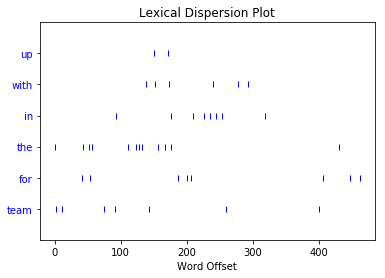
\includegraphics[width=.9\linewidth]{./obipy-resources/l01HMt.png}
\end{center}
\end{enumerate}
\subsubsection{generation\hfill{}\textsc{test}}
\label{sec:org94d06ce}
\begin{verbatim}
text.generate(["The", "job", "is", "for", "data", "team"])
\end{verbatim}

\subsubsection{normalizing}
\label{sec:orgcc09771}
\begin{enumerate}
\item steaming
\label{sec:org7b4f46e}
\item lemmatization
\label{sec:orgfb3de67}
\end{enumerate}
\subsubsection{vocabulary}
\label{sec:org01b4546}
\begin{enumerate}
\item sorted set
\label{sec:org078b7af}
\begin{verbatim}
sorted(set(text))
\end{verbatim}

\begin{verbatim}
['17',
'2008',
'23',
'3',
'40',
'5',
'<',
'a',
'able',
'about',
'academic',
'across',
'active',
'adapt',
'additional',
'advertising',
'all',
'also',
'an',
'analysis',
'analysts',
'analytical',
'analytics',
'analyzing',
'and',
'anja',
'are',
'area',
'art',
'as',
'aspects',
'assistance',
'at',
'atmosphere',
'attitude',
'available',
'backgrounds',
'basis',
'behavior',
'beverages',
'bieten',
'brands',
'bringing',
'building',
'business',
'but',
'celebrate',
'centrally',
'challenges',
'change',
'changing',
'choose',
'closely',
'coaching',
'com',
'come',
'commerce',
'committed',
'communicating',
'comparable',
'competitive',
'computer',
'conflicts',
'connecting',
'context',
'contribute',
'crm',
'customer',
'customers',
'daily',
'data',
'databases',
'de',
'decided',
'decisions',
'deep',
'department',
'develop',
'developing',
'development',
'different',
'digital',
'direct',
'discount',
'discounts',
'diverse',
'diversity',
'drive',
'e',
'easily',
'economics',
'effectively',
'ein',
'einkaufserlebnis',
'employee',
'employment',
'empowerment',
'enable',
'entire',
'environment',
'equipment',
'equivalent',
'europas',
'europe',
'experience',
'expertise',
'experts',
'external',
'fashion',
'fast',
'feedback',
'field',
'flexible',
'focus',
'for',
'foundation',
'free',
'from',
'fruits',
'full',
'führende',
'g',
'getting',
'great',
'groups',
'have',
'head',
'health',
'help',
'holidays',
'https',
'ideally',
'impact',
'in',
'independently',
'information',
'innovations',
'insights',
'inspiring',
'intelligence',
'interests',
'internal',
'international',
'internationals',
'into',
'is',
'ist',
'it',
'its',
'junior',
'keep',
'knowledge',
'kunden',
'languages',
'lay',
'lead',
'leading',
'located',
'logistics',
'long',
'look',
'looking',
'lounge',
'mail',
'managing',
'many',
'markets',
'mathematics',
'means',
'members',
'mentoring',
'merit',
'methods',
'million',
'models',
'more',
'most',
'municipality',
'name',
'need',
'needed',
'new',
'not',
'of',
'off',
'offering',
'offerings',
'offices',
'on',
'online',
'only',
'opensource',
'opportunities',
'or',
'other',
'our',
'out',
'paced',
'partners',
'perks',
'personal',
'perspectives',
'platform',
'plattform',
'positive',
'potential',
'priorities',
'proactive',
'public',
'python',
'qualifications',
'questions',
'quick',
'r',
'radar',
're',
'recruiter',
'related',
'relevant',
'relocation',
'reports',
'represent',
'research',
'responsibility',
'run',
's',
'salary',
'science',
'segment',
'seit',
'senior',
'services',
'sets',
'share',
'shop',
'shopping',
'showcases',
'similar',
'size',
'skill',
'skills',
'solutions',
'solve',
'spierling',
'sports',
'sql',
'stakeholders',
'state',
'statistical',
'statistics',
'strategy',
'structures',
'subject',
'tailored',
'team',
'teams',
'tech',
'technical',
'term',
'than',
'that',
'the',
'their',
'them',
'things',
'thinking',
'through',
'time',
'times',
'to',
'toe',
'together',
'too',
'top',
'transforming',
'transport',
'trust',
'umfassendes',
'understanding',
'unseren',
'up',
'use',
'user',
'using',
'valuable',
'variety',
'volunteering',
'warehouse',
'ways',
'we',
'well',
'what',
'where',
'which',
'will',
'wir',
'with',
'work',
'working',
'workplace',
'x',
'years',
'you',
'your',
'zalando']
\end{verbatim}
\item lexical richness
\label{sec:org27063ea}
\begin{enumerate}
\item tryout
\label{sec:org281f1b3}
\begin{verbatim}
len(text) / len(set(text))
\end{verbatim}

\item function
\label{sec:org33caec5}
\begin{verbatim}
def lexical_diversity(text):
    return len(text) / len(set(text))
\end{verbatim}

\begin{verbatim}
1.6950819672131148
\end{verbatim}
\end{enumerate}
\item specific word
\label{sec:org9a047d8}
\begin{enumerate}
\item tryout
\label{sec:orgecc3d34}
\begin{verbatim}
100 * text.count('for') / len(text)
\end{verbatim}

\begin{verbatim}
1.5473887814313345
\end{verbatim}
\item functyion
\label{sec:orge20b842}
\begin{verbatim}
def word_percentage(word):
    return 100 * text.count(word) / len(text)
\end{verbatim}
\end{enumerate}
\end{enumerate}

\subsubsection{{\bfseries\sffamily TODO} Build a corpus !}
\label{sec:orgde43555}

\begin{enumerate}
\item sklearn
\label{sec:org38809d1}
\begin{verbatim}
docs = df['desc']

tfs = tfidf.fit_transform(docs)
\end{verbatim}
\end{enumerate}
\end{document}